\documentclass[12pt,a4paper]{article}
% ========== PACKAGES ==========
\usepackage[utf8]{inputenc}
\usepackage[T5]{fontenc}
\usepackage[vietnamese]{babel}
\usepackage{lmodern}
\setlength{\headheight}{14pt}
\usepackage{geometry}
\usepackage{graphicx}
\usepackage{amsmath}
\usepackage{amssymb}
\usepackage{booktabs}
\usepackage{array}
\usepackage{multirow}
\usepackage{tabularx}
\usepackage{fancyhdr}
\usepackage{tikz}
\usetikzlibrary{positioning}
\usepackage{pgfplots}
\pgfplotsset{compat=1.18}
\usepackage{eso-pic}
\usepackage{xcolor}
\usepackage{hyperref}
\usepackage{titlesec}
\usepackage{enumitem}
\usepackage{lastpage}
\usepackage{float}
\usepackage[table]{xcolor}
\usepackage[most]{tcolorbox}
\usepackage{listings}
\usepackage{caption}

% ========== LISTINGS CONFIG ==========
\definecolor{codegreen}{rgb}{0,0.6,0}
\definecolor{codegray}{rgb}{0.5,0.5,0.5}
\definecolor{codepurple}{rgb}{0.58,0,0.82}
\definecolor{codebg}{rgb}{0.95,0.95,0.92}

\lstdefinestyle{pythonstyle}{
    backgroundcolor=\color{codebg},
    commentstyle=\color{codegreen},
    keywordstyle=\color{blue},
    numberstyle=\tiny\color{codegray},
    stringstyle=\color{codepurple},
    basicstyle=\ttfamily\footnotesize,
    breakatwhitespace=false,
    breaklines=true,
    captionpos=b,
    keepspaces=true,
    numbers=left,
    numbersep=5pt,
    showspaces=false,
    showstringspaces=false,
    showtabs=false,
    tabsize=2,
    language=Python
}
\lstset{style=pythonstyle}

\definecolor{rowgray}{gray}{0.9}
\newtcolorbox{formulabox}{
    colback=blue!5!white,
    colframe=blue!75!black,
    left=5pt, right=5pt, top=5pt, bottom=5pt,
    sharp corners, boxrule=0.5pt
}


% ========== PAGE GEOMETRY ==========
\geometry{
    a4paper,
    top=2.5cm,
    bottom=2.5cm,
    left=3cm,
    right=2.5cm
}

% ========== BORDER (CHỈ TRANG ĐẦU) ==========
\newcommand{\firstpageborder}{%
\begin{tikzpicture}[remember picture, overlay]
\draw[line width=2pt, black]
            ([xshift=1.2cm, yshift=-1.2cm]current page.north west)
            rectangle
            ([xshift=-1.2cm, yshift=1.2cm]current page.south east);
\draw[line width=0.5pt, black]
            ([xshift=1.4cm, yshift=-1.4cm]current page.north west)
            rectangle
            ([xshift=-1.4cm, yshift=1.4cm]current page.south east);
\end{tikzpicture}%
}

% ========== WATERMARK ẢNH (CHỈ TRANG ĐẦU) ==========
\newcommand{\firstpagewatermark}{%
\begin{tikzpicture}[remember picture, overlay]
\node[opacity=0.3] at (current page.center) {

\includegraphics[width=20cm]{logo.png}
        };
\end{tikzpicture}%
}

% ========== HEADER / FOOTER ==========
\pagestyle{fancy}
\fancyhf{}
\renewcommand{\headrulewidth}{0.4pt}
\renewcommand{\footrulewidth}{0.4pt}
\fancyhead[L]{\small Nhập môn trí tuệ nhân tạo}
\fancyhead[R]{\small Nhóm: 10}
\fancyfoot[C]{\small Trang \thepage\ / \pageref{LastPage}}
\fancypagestyle{firstpage}{%
\fancyhf{}
\renewcommand{\headrulewidth}{0pt}
\renewcommand{\footrulewidth}{0pt}
}

% ========== SECTION FORMAT ==========
\titleformat{\section}{\large\bfseries}{}{0em}{}[\titlerule]
\titleformat{\subsection}{\normalsize\bfseries}{}{0em}{}

% ========== DOCUMENT ==========
\begin{document}

% ===== TRANG ĐẦU =====
\thispagestyle{firstpage}
\firstpageborder
\firstpagewatermark
\vspace*{1cm}
\begin{center}
\begin{minipage}{0.15\textwidth}

\includegraphics[width=\linewidth]{logo.png}
\end{minipage}
\hspace{0.3cm}
\begin{minipage}{0.8\textwidth}
\centering
        {\normalsize\bfseries TRƯỜNG ĐẠI HỌC KHOA HỌC TỰ NHIÊN \\
        ĐẠI HỌC QUỐC GIA THÀNH PHỐ HỒ CHÍ MINH}
\end{minipage}
\end{center}

\begin{center}
\rule{0.6\textwidth}{0.5pt}\\[0.8cm]
    {\LARGE\bfseries BÁO CÁO CUỐI KỲ}\\[0.5cm]
    {\large\bfseries NHẬP MÔN TRÍ TUỆ NHÂN TẠO}\\[0.8cm]
\rule{0.6\textwidth}{0.5pt}\\[1cm]
    {\normalsize\textbf{GVPT:} ThS. Nguyễn Quốc Khoa}\\[2cm]
\end{center}

\begin{center}
\begin{tabular}{ll}
\textbf{Ca:} & 1 \\[0.3cm]
\textbf{Họ và tên SV:} & Huỳnh Ngọc Huy \\[0.3cm]
\textbf{MSSV:} & 24200087 \\[0.3cm]
\textbf{Thành viên nhóm:} & Huỳnh Ngọc Huy - 24200087\\
\textbf{ } & Choi Won Seok - 24200032
\end{tabular}
\end{center}

\newpage
% ======================================================================
%                      MỤC LỤC
% ======================================================================
\tableofcontents
\newpage

% ======================================================================
%                      DANH SÁCH HÌNH & BẢNG
% ======================================================================
\listoffigures
\listoftables
\newpage

% ======================================================================
%                   1. GIỚI THIỆU
% ======================================================================
\section{Giới Thiệu}

\subsection{Đặt Vấn Đề}
Nhận diện biển báo giao thông là một thành phần quan trọng trong hệ thống xe tự lái và hệ thống hỗ trợ người lái tiên tiến (ADAS). Mục tiêu là tự động phân loại ảnh biển báo giao thông vào đúng danh mục (ví dụ: giới hạn tốc độ, dừng, nhường đường) từ hình ảnh camera thu được từ xe.

Bài toán này gặp nhiều thách thức do sự thay đổi về điều kiện ánh sáng, vật che khuất, mờ chuyển động và thời tiết khác nhau. Các phương pháp truyền thống như trích xuất đặc trưng thủ công (HOG, SIFT) kết hợp SVM gặp khó khăn khi xử lý 43 loại biển báo khác nhau với chất lượng ảnh không đồng nhất.

\subsection{Mục Tiêu Đề Án}
Đề án này xây dựng một hệ thống nhận diện biển báo giao thông sử dụng Convolutional Neural Network (CNN) với TensorFlow/Keras trên bộ dữ liệu German Traffic Sign Recognition Benchmark (GTSRB). Mô hình phải xác định chính xác mỗi ảnh đầu vào thuộc 1 trong 43 loại biển báo.

Các mục tiêu cụ thể:
\begin{enumerate}[leftmargin=*]
    \item Xây dựng pipeline hoàn chỉnh từ đọc dữ liệu đến huấn luyện và đánh giá mô hình CNN.
    \item Xử lý vấn đề mất cân bằng dữ liệu giữa các lớp bằng class weights.
    \item Thử nghiệm và so sánh nhiều thuật toán/kiến trúc khác nhau.
    \item Đánh giá chi tiết bằng classification report (precision, recall, F1-score).
    \item Xây dựng công cụ inference cho ảnh đơn và thư mục ảnh.
\end{enumerate}

\subsection{Phương Pháp Tiếp Cận}
Chúng tôi áp dụng phương pháp học sâu có giám sát theo quy trình 8 bước:

\begin{enumerate}[label=\textbf{Bước \arabic*:},leftmargin=*]
    \item Đọc và tiền xử lý ảnh biển báo giao thông từ bộ dữ liệu GTSRB.
    \item Phân tích phân phối lớp và tính class weights để xử lý mất cân bằng.
    \item Chuẩn hóa dữ liệu về khoảng $[0, 1]$ và áp dụng data augmentation trong quá trình huấn luyện.
    \item Mã hóa nhãn bằng one-hot encoding cho bài toán phân loại đa lớp.
    \item Chia dữ liệu thành tập huấn luyện (80\%) và tập kiểm tra (20\%).
    \item Xây dựng kiến trúc CNN và biên dịch mô hình với Adam optimizer.
    \item Huấn luyện mô hình trong 10 epoch và đánh giá trên tập kiểm tra.
    \item So sánh kết quả giữa các thuật toán khác nhau.
\end{enumerate}

% ======================================================================
%                   2. MÔ TẢ BỘ DỮ LIỆU
% ======================================================================
\section{Mô Tả Bộ Dữ Liệu}

\subsection{Tổng Quan về GTSRB}
German Traffic Sign Recognition Benchmark (GTSRB) chứa hơn 50.000 ảnh biển báo giao thông được chia thành 43 lớp riêng biệt. Mỗi lớp tương ứng với một loại biển báo giao thông của Đức. Đây là bộ dữ liệu chuẩn được sử dụng rộng rãi trong nghiên cứu nhận diện biển báo.

\subsection{Cấu Trúc Thư Mục}
Bộ dữ liệu được tổ chức dưới dạng cây thư mục:

\begin{verbatim}
gtsrb/
+-- 0/          # Gioi han toc do 20 km/h
+-- 1/          # Gioi han toc do 30 km/h
+-- 2/          # Gioi han toc do 50 km/h
...
+-- 42/         # Het han che vuot (xe tai)
\end{verbatim}

Mỗi thư mục con chứa các tập tin ảnh PNG/PPM với kích thước khác nhau, tất cả thuộc cùng một loại biển báo. Tên thư mục (0--42) đóng vai trò là nhãn nguyên cho danh mục đó.

\subsection{Đặc Điểm Dữ Liệu}
\begin{itemize}
    \item \textbf{Số lớp:} 43
    \item \textbf{Định dạng ảnh:} PPM / PNG (màu RGB)
    \item \textbf{Kích thước ảnh thay đổi:} Cần thay đổi kích thước trước khi đưa vào mạng. Cả hai chương trình \texttt{trafficsign.py} và \texttt{trafficsign\_new.py} đều resize ảnh về $30 \times 30$.
    \item \textbf{Kích thước đầu vào:} $30 \times 30 \times 3$ cho tất cả mô hình (riêng MobileNetV2 resize lên $96 \times 96$ bên trong mô hình).
\end{itemize}

\subsection{Phân Tích Mất Cân Bằng Dữ Liệu}
Bộ dữ liệu GTSRB có sự mất cân bằng đáng kể giữa các lớp:

\begin{table}[H]
\centering
\begin{tabular}{@{}lcccc@{}}
\toprule
\textbf{Chỉ số} & \textbf{Giá trị} \\ \midrule
Lớp ít ảnh nhất   & Lớp 0 (150 ảnh) \\
Lớp nhiều ảnh nhất & Lớp 1 (1500 ảnh) \\
Tổng số ảnh       & 26.640 \\
Tỷ lệ mất cân bằng (max/min) & 10:1 \\ \bottomrule
\end{tabular}
\caption{Phân tích sự mất cân bằng dữ liệu GTSRB.}
\label{tab:imbalance}
\end{table}

Sự chênh lệch lớn (lớp 1 có gấp 10 lần lớp 0) có thể ảnh hưởng tiêu cực đến hiệu suất mô hình: mô hình sẽ thiên vị dự đoán các lớp đa số và bỏ qua các lớp thiểu số. Đây là vấn đề quan trọng cần được xử lý để đạt điểm cao (mức 9 điểm).

\subsection{Biểu Đồ Phân Phối Lớp}

\begin{figure}[H]
\centering
\begin{tikzpicture}
\begin{axis}[
    width=0.95\textwidth,
    height=8cm,
    xlabel={Mã lớp},
    ylabel={Số lượng ảnh},
    xmin=0, xmax=43,
    ymin=0, ymax=1600,
    ybar,
    bar width=3pt,
    xtick={0,5,10,15,20,25,30,35,40},
    xticklabels={0,5,10,15,20,25,30,35,40},
    grid=major,
    title={Phân phối dữ liệu GTSRB theo từng lớp (43 lớp)},
]
\addplot[blue, fill=blue!30] coordinates {
    (0,150)(1,1500)(2,1500)(3,960)(4,1320)(5,1260)(6,300)(7,960)
    (8,960)(9,990)(10,1350)(11,900)(12,1410)(13,1440)(14,540)
    (15,420)(16,300)(17,750)(18,810)(19,150)(20,240)(21,240)
    (22,270)(23,360)(24,180)(25,1020)(26,420)(27,180)(28,360)
    (29,180)(30,300)(31,540)(32,180)(33,480)(34,300)(35,810)
    (36,270)(37,150)(38,1380)(39,210)(40,240)(41,180)(42,180)
};
\addplot[red, thick, sharp plot] coordinates {
    (0,620)(42,620)
};
\addlegendentry{Số ảnh mỗi lớp}
\addlegendentry{Trung bình (620 ảnh/lớp)}
\end{axis}
\end{tikzpicture}
\caption{Biểu đồ phân phối số lượng ảnh trên 43 lớp của GTSRB. Đường đỏ thể hiện mức trung bình 619 ảnh/lớp. Các lớp 0, 19, 37--42 có ít hơn 200 ảnh, trong khi lớp 1 có đến 1500 ảnh.}
\label{fig:class_dist}
\end{figure}

Sự mất cân bằng thể hiện rõ qua biểu đồ: các lớp từ 0--14 (nhóm biển báo giới hạn tốc độ) chiếm phần lớn dữ liệu, trong khi các lớp từ 37--42 (nhóm biển báo hết hạn chế) chỉ có 150--165 ảnh mỗi lớp. Nếu không xử lý, mô hình sẽ học rất tốt nhóm đa số nhưng gần như "mù" với nhóm thiểu số. Đây là động lực chính để áp dụng class weights.

% ======================================================================
%                   3. PHƯƠNG PHÁP THỰC HIỆN
% ======================================================================
\section{Phương Pháp Thực Hiện}

\subsection{Cấu Hình Toàn Cục}
Các siêu tham số được định nghĩa ở mức module:

\begin{table}[H]
\centering
\begin{tabular}{@{}lll@{}}
\toprule
\textbf{Hằng số} & \textbf{Giá trị} & \textbf{Mô tả} \\ \midrule
\texttt{EPOCHS}         & 10    & Số epoch huấn luyện tối đa \\
\texttt{IMG\_WIDTH}     & 30 & Chiều rộng ảnh đích (cả hai chương trình) \\
\texttt{IMG\_HEIGHT}    & 30 & Chiều cao ảnh đích (cả hai chương trình) \\
\texttt{NUM\_CATEGORIES}& 43    & Số lớp biển báo \\
\texttt{TEST\_SIZE}     & 0.2   & Tỷ lệ dữ liệu kiểm tra (80\% train / 20\% test) \\
\texttt{BATCH\_SIZE}    & 32    & Kích thước batch (chỉ \texttt{trafficsign\_new.py}) \\ \bottomrule
\end{tabular}
\caption{Siêu tham số toàn cục.}
\label{tab:hyperparams}
\end{table}

\subsection{Bước 1: Đọc Dữ Liệu -- \texttt{load\_data()}}

Hàm \texttt{load\_data(data\_dir)} duyệt qua tất cả 43 thư mục con, đọc từng ảnh bằng OpenCV, thay đổi kích thước về $30 \times 30$, và trả về tuple \texttt{(images, labels)}.

\subsubsection*{Thuật Toán}
\begin{enumerate}[leftmargin=*]
    \item Khởi tạo hai danh sách rỗng: \texttt{images = []} và \texttt{labels = []}.
    \item Lặp \texttt{category} từ 0 đến \texttt{NUM\_CATEGORIES - 1} (tức 0--42):
    \begin{enumerate}
        \item Tạo đường dẫn \texttt{category\_path = data\_dir/str(category)}.
        \item Liệt kê tất cả tập tin trong thư mục đó bằng \texttt{os.listdir()}.
        \item Với mỗi tập tin \texttt{filename} (chỉ xử lý các đuôi .png, .jpg, .jpeg, .ppm, .bmp):
        \begin{enumerate}
            \item Đọc ảnh: \texttt{cv2.imread(img\_path)}.
            \item Nếu ảnh bị hỏng (\texttt{img is None}), bỏ qua và tăng biến đếm \texttt{skipped}.
            \item Chuyển đổi BGR (OpenCV) sang RGB: \texttt{cv2.cvtColor(img, cv2.COLOR\_BGR2RGB)}.
            \item Thay đổi kích thước: \texttt{cv2.resize(img, (IMG\_WIDTH, IMG\_HEIGHT))}.
            \item Chuẩn hóa về $[0,1]$: \texttt{img.astype(np.float32) / 255.0}.
            \item Thêm ảnh đã xử lý vào \texttt{images}.
            \item Thêm nhãn nguyên \texttt{category} vào \texttt{labels}.
        \end{enumerate}
    \end{enumerate}
    \item Trả về \texttt{(images, labels)}.
\end{enumerate}

\subsubsection*{Cài Đặt}
\begin{lstlisting}[language=Python, caption={Hàm \texttt{load\_data()} hoàn chỉnh.}, label=lst:load_data]
def load_data(data_dir):
    images = []
    labels = []
    skipped = 0

    for category in range(NUM_CATEGORIES):
        category_path = os.path.join(data_dir, str(category))
        if not os.path.isdir(category_path):
            continue

        for filename in os.listdir(category_path):
            # Only process image files; skip CSVs and other non-image files
            if not filename.lower().endswith((".png", ".jpg", ".jpeg", ".ppm", ".bmp")):
                continue

            img_path = os.path.join(category_path, filename)
            img = cv2.imread(img_path)

            # Bo qua file bi hong / khong doc duoc
            if img is None:
                skipped += 1
                continue

            # Chuyen BGR (OpenCV) -> RGB de dong bo voi inference
            img = cv2.cvtColor(img, cv2.COLOR_BGR2RGB)
            img = cv2.resize(img, (IMG_WIDTH, IMG_HEIGHT))

            # Chuan hoa ve [0, 1] ngay tai day
            img = img.astype(np.float32) / 255.0

            images.append(img)
            labels.append(category)

    if skipped:
        print(f"Skipped {skipped} unreadable file(s).")

    return images, labels
\end{lstlisting}

Điểm khác biệt so với phiên bản cơ bản: \texttt{trafficsign\_new.py} thêm bộ lọc đuôi file (\texttt{.endswith(...)}) để bỏ qua các file CSV và file không phải ảnh, giúp quá trình đọc dữ liệu an toàn hơn.

\subsection{Bước 2: Phân Tích và Xử Lý Mất Cân Bằng -- Class Weights (9 điểm)}

Đây là kỹ thuật then chốt để đạt mức 9 điểm. Cả hai chương trình \texttt{trafficsign.py} và \texttt{trafficsign\_new.py} đều sử dụng \texttt{sklearn.utils.class\_weight.compute\_class\_weight} với chế độ \texttt{"balanced"} để tính trọng số cho mỗi lớp.

\subsubsection*{Công Thức}
Trọng số cho lớp $c$ được tính theo công thức:
\begin{equation}
    w_c = \frac{N_{\text{total}}}{N_{\text{classes}} \times N_c}
\end{equation}

Trong đó:
\begin{itemize}
    \item $N_{\text{total}} = 26.640$: tổng số mẫu trong tập dữ liệu.
    \item $N_{\text{classes}} = 43$: số lượng lớp.
    \item $N_c$: số mẫu trong lớp $c$.
\end{itemize}

Lớp càng ít mẫu thì trọng số càng cao, buộc mô hình phải chú ý nhiều hơn đến các lớp thiểu số trong quá trình huấn luyện.

\subsubsection*{Cài Đặt}
\begin{lstlisting}[language=Python, caption={Tính class weights xử lý mất cân bằng.}, label=lst:class_weights]
from sklearn.utils import class_weight

# labels_int contains integer labels (0-42) for all images
class_weights_array = class_weight.compute_class_weight(
    class_weight="balanced",
    classes=np.unique(labels_int),
    y=labels_int
)
class_weight_dict = {i: class_weights_array[i] for i in range(NUM_CATEGORIES)}

# Pass to model.fit()
model.fit(x_train, y_train, ..., class_weight=class_weight_dict)
\end{lstlisting}

\subsubsection*{Phân Tích Trọng Số}
\begin{itemize}
    \item Lớp 0 (150 ảnh): $w_0 = 26.640 / (43 \times 150) \approx 4.13$ -- trọng số cao nhất.
    \item Lớp 1 (1500 ảnh): $w_1 = 26.640 / (43 \times 1500) \approx 0.41$ -- trọng số thấp nhất.
    \item Tỷ lệ trọng số max/min: $\approx 10:1$, phản ánh chính xác tỷ lệ mất cân bằng.
\end{itemize}

\subsection{Bước 3: Chuẩn Hóa Dữ Liệu và Data Augmentation}

\subsubsection*{Chuẩn Hóa}
Chuẩn hóa giá trị pixel về khoảng $[0, 1]$ được thực hiện trực tiếp trong hàm \texttt{load\_data()} để đảm bảo nhất quán giữa huấn luyện và inference:

\begin{lstlisting}[language=Python]
img = img.astype(np.float32) / 255.0
\end{lstlisting}

Việc chuẩn hóa giúp huấn luyện ổn định và nhanh hội tụ hơn vì giá trị pixel nằm trong khoảng nhỏ, gradient không bị bùng nổ.

\subsubsection*{Data Augmentation (chỉ \texttt{trafficsign\_new.py})}

Trong quá trình huấn luyện, \texttt{trafficsign\_new.py} sử dụng \texttt{ImageDataGenerator} để tạo các biến thể của ảnh huấn luyện theo thời gian thực (real-time augmentation), giúp mô hình khái quát hóa tốt hơn:

\begin{lstlisting}[language=Python, caption={Cấu hình Data Augmentation.}, label=lst:augmentation]
datagen = ImageDataGenerator(
    rotation_range=10,        # Xoay ngau nhien +-10 do
    zoom_range=0.15,           # Zoom ngau nhien 0-15%
    width_shift_range=0.1,     # Dich ngang 10%
    height_shift_range=0.1,    # Dich doc 10%
    shear_range=0.1,           # Bien dang shear 10%
    horizontal_flip=False,     # KHONG lat ngang -- bien bao khong doi xung
    fill_mode="nearest"        # Dien pixel thieu bang gia tri gan nhat
)
\end{lstlisting}

\textbf{Lưu ý quan trọng:} \texttt{horizontal\_flip=False} vì biển báo giao thông không đối xứng ngang -- việc lật ngang sẽ tạo ra ảnh không có thật (ví dụ: biển báo rẽ phải thành rẽ trái).

Data augmentation được áp dụng thông qua \texttt{datagen.flow(x\_train, y\_train, batch\_size=BATCH\_SIZE)} khi gọi \texttt{model.fit()}, đảm bảo mỗi epoch mô hình nhìn thấy các biến thể khác nhau của cùng một ảnh.

\subsubsection*{L2 Regularization (Model B)}
Model B sử dụng L2 regularization (weight decay) với hệ số $\lambda=0.001$ trên tất cả các lớp Conv2D và Dense. L2 regularization thêm thành phần phạt vào hàm mất mát:
\begin{equation}
    \mathcal{L}_{\text{total}} = \mathcal{L}_{\text{CE}} + \lambda \sum_{w} w^2
\end{equation}

Các trọng số lớn bị phạt, khuyến khích mô hình học các trọng số nhỏ và phân bố đều -- giúp giảm overfitting.

\subsection{Bước 4: Mã Hóa Nhãn (One-Hot Encoding)}

Nhãn nguyên được chuyển đổi thành vector one-hot 43 chiều:

\begin{lstlisting}[language=Python]
labels_cat = tf.keras.utils.to_categorical(labels_int, NUM_CATEGORIES)
\end{lstlisting}

Mỗi nhãn $y \in \{0, 1, \dots, 42\}$ trở thành vector 43 chiều, chỉ vị trí $y$ là 1, các vị trí khác là 0.

\textbf{Ví dụ:} Nhãn \texttt{3} trở thành \texttt{[0, 0, 0, 1, 0, 0, ..., 0]} (độ dài 43).

Đây là định dạng bắt buộc cho hàm mất mát categorical cross-entropy.

\subsection{Bước 5: Chia Dữ Liệu}

Dữ liệu được chia ngẫu nhiên với \texttt{random\_state=42} để đảm bảo khả năng tái lập:

\begin{lstlisting}[language=Python]
x_train, x_test, y_train, y_test = train_test_split(
    np.array(images), labels_cat, test_size=TEST_SIZE, random_state=42
)
\end{lstlisting}

\begin{itemize}
    \item \textbf{Tập huấn luyện (80\%):} $\sim$21.312 ảnh -- dùng để điều chỉnh trọng số mô hình.
    \item \textbf{Tập kiểm tra (20\%):} $\sim$5.328 ảnh -- dùng để đánh giá khả năng tổng quát hóa.
\end{itemize}

\subsection{Bước 6: Xây Dựng Mô Hình CNN}

\subsubsection*{Kiến Trúc Baseline CNN (Model A)}

Mô hình sử dụng 2 khối tích chập kép (double-Conv), mỗi khối gồm 2 lớp Conv2D liên tiếp với kích thước kernel khác nhau ($5\times5$ cho khối 1, $3\times3$ cho khối 2), sau đó MaxPooling2D + Dropout(0.25), rồi Flatten, Dense(256), Dropout(0.5) và Softmax:

\begin{table}[H]
\centering
\begin{tabular}{@{}lll@{}}
\toprule
\textbf{Lớp (loại)} & \textbf{Cấu hình} & \textbf{Kích thước đầu ra} \\ \midrule
Conv2D + ReLU     & 32 filters, $5\times5$, valid padding  & $(26, 26, 32)$  \\
Conv2D + ReLU     & 32 filters, $5\times5$, valid padding  & $(22, 22, 32)$  \\
MaxPooling2D      & $2\times2$                             & $(11, 11, 32)$  \\
Dropout           & rate = 0.25                            & $(11, 11, 32)$  \\
Conv2D + ReLU     & 64 filters, $3\times3$, valid padding  & $(9, 9, 64)$    \\
Conv2D + ReLU     & 64 filters, $3\times3$, valid padding  & $(7, 7, 64)$    \\
MaxPooling2D      & $2\times2$                             & $(3, 3, 64)$    \\
Dropout           & rate = 0.25                            & $(3, 3, 64)$    \\
Flatten           & --                                     & $(576)$          \\
Dense + ReLU      & 256 units                              & $(256)$          \\
Dropout           & rate = 0.5                             & $(256)$          \\
Dense + Softmax   & 43 units (đầu ra)                      & $(43)$           \\ \bottomrule
\end{tabular}
\caption{Kiến trúc Baseline CNN. Đầu vào $(30, 30, 3)$.}
\label{tab:cnn_arch}
\end{table}

\begin{figure}[H]
\centering
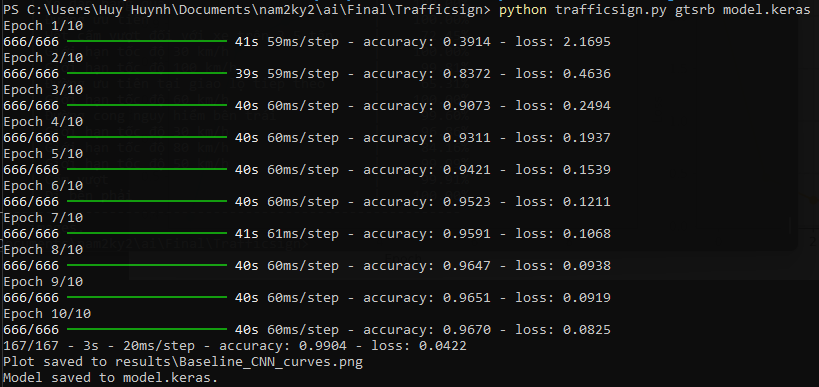
\includegraphics[width=0.85\textwidth]{../ImageReport_new/model_keras.png}
\caption{Sơ đồ kiến trúc mô hình CNN hiển thị qua \texttt{model.summary()} và \texttt{tf.keras.utils.plot\_model()}. Các tầng Conv2D, MaxPooling2D, Dropout, Flatten, Dense được hiển thị với kích thước đầu ra và số tham số.}
\label{fig:model_keras}
\end{figure}

\subsubsection*{Cài Đặt}
\begin{lstlisting}[language=Python, caption={Hàm \texttt{build\_baseline\_cnn()} -- Model A.}, label=lst:model_a]
def build_baseline_cnn():
    model = tf.keras.models.Sequential([
        tf.keras.layers.Input(shape=(IMG_WIDTH, IMG_HEIGHT, 3)),

        # --- Block 1: 5x5 filters for general features ---
        tf.keras.layers.Conv2D(32, (5, 5), activation="relu"),
        tf.keras.layers.Conv2D(32, (5, 5), activation="relu"),
        tf.keras.layers.MaxPooling2D(pool_size=(2, 2)),
        tf.keras.layers.Dropout(0.25),

        # --- Block 2: 3x3 filters for specific features ---
        tf.keras.layers.Conv2D(64, (3, 3), activation="relu"),
        tf.keras.layers.Conv2D(64, (3, 3), activation="relu"),
        tf.keras.layers.MaxPooling2D(pool_size=(2, 2)),
        tf.keras.layers.Dropout(0.25),

        # Flatten + Hidden + Dropout + Output
        tf.keras.layers.Flatten(),
        tf.keras.layers.Dense(256, activation="relu"),
        tf.keras.layers.Dropout(0.5),
        tf.keras.layers.Dense(NUM_CATEGORIES, activation="softmax"),
    ])
    model.compile(optimizer="adam",
                  loss="categorical_crossentropy",
                  metrics=["accuracy"])
    return model
\end{lstlisting}

\subsubsection*{Giải Thích Thiết Kế Chi Tiết}

\textbf{1. Double-Conv trong mỗi khối:}

Mỗi khối sử dụng 2 lớp Conv2D liên tiếp thay vì 1 lớp đơn:
\begin{itemize}
    \item Hai lớp Conv2D(32) liên tiếp có vùng tiếp nhận hiệu quả (effective receptive field) tương đương một lớp Conv2D với kernel $9\times9$, nhưng với ít tham số hơn và nhiều tính phi tuyến hơn (2 lần ReLU).
    \item \textbf{Khối 1 (5x5 kernels):} Kernel $5\times5$ bắt được các đặc trưng tổng quát trên ảnh $30\times30$ -- hình dạng tròn/tam giác/vuông của biển báo.
    \item \textbf{Khối 2 (3x3 kernels):} Kernel $3\times3$ bắt các chi tiết cụ thể hơn -- ký hiệu, chữ số bên trong biển báo.
    \item \textbf{Số filter tăng dần (32$\to$64):} Các lớp đầu học đặc trưng cấp thấp (cạnh, góc, màu sắc). Các lớp sau tổ hợp chúng thành đặc trưng cấp cao (hình dạng biển báo, biểu tượng).
\end{itemize}

\textbf{2. Tầng Gộp (MaxPooling2D) -- Giảm Chiều:}
\begin{equation}
    \text{MaxPool}(I)_{i,j} = \max_{m,n \in \{0,1\}} I(2i+m, 2j+n)
\end{equation}
\begin{itemize}
    \item \textbf{Kích thước pool $2\times2$:} Giảm kích thước không gian đi một nửa sau mỗi khối: $30\to15$ (sau Conv), rồi $11\to5$ (khối 1), $3\to1$ (khối 2) -- nhưng kích thước thực tế phụ thuộc vào padding. Với valid padding, luồng không gian là: $30\to26\to22\to11\to9\to7\to3$.
    \item \textbf{Tính bất biến dịch chuyển:} MaxPooling giúp mô hình nhận diện đặc trưng ngay cả khi chúng bị dịch chuyển nhẹ -- quan trọng vì biển báo không luôn ở chính giữa khung hình.
\end{itemize}

\textbf{3. Hàm Kích Hoạt ReLU (Rectified Linear Unit):}
\begin{equation}
    \text{ReLU}(x) = \max(0, x)
\end{equation}
\begin{itemize}
    \item \textbf{Ưu điểm:} Đạo hàm đơn giản (0 hoặc 1), không bão hòa như sigmoid/tanh, giúp gradient lan truyền hiệu quả qua nhiều lớp (tránh vanishing gradient).
    \item \textbf{Tính thưa (sparsity):} Khoảng 50\% neuron có đầu ra = 0, tạo ra biểu diễn thưa và hiệu quả.
\end{itemize}

\textbf{4. Tầng Flatten -- Cầu Nối CNN-Dense:}

Chuyển tensor 3D thành vector 1D: $(3, 3, 64) \to (576,)$. Đây là vector đặc trưng tổng hợp chứa toàn bộ thông tin trích xuất từ ảnh.

\textbf{5. Tầng Kết Nối Đầy Đủ (Dense) -- Phân Loại:}

Dense(256) thực hiện phép biến đổi tuyến tính + ReLU:
\begin{equation}
    \mathbf{h} = \text{ReLU}(\mathbf{W} \cdot \mathbf{x} + \mathbf{b})
\end{equation}
Với $\mathbf{W} \in \mathbb{R}^{256 \times 576}$ và $\mathbf{b} \in \mathbb{R}^{256}$.

\textbf{6. Dropout(0.25) sau mỗi khối Conv và Dropout(0.5) trước đầu ra:}

Trong quá trình huấn luyện, mỗi neuron có xác suất $p$ bị tắt (đầu ra = 0). Dropout nhẹ (0.25) sau các lớp Conv giúp chống overfitting ở mức đặc trưng không gian. Dropout mạnh hơn (0.5) ở lớp Dense chống overfitting ở mức kết hợp đặc trưng toàn cục.

Việc chia cho $1-p$ (inverted dropout) đảm bảo tổng activation không đổi khi chuyển từ train sang test. Tại test time, tất cả neuron đều hoạt động.

\textbf{7. Softmax -- Đầu Ra Phân Loại:}
\begin{equation}
    P(y = c \mid \mathbf{x}) = \frac{e^{z_c}}{\sum_{j=1}^{43} e^{z_j}}
\end{equation}
Chuyển vector logits $\mathbf{z}$ thành phân phối xác suất trên 43 lớp. Lớp dự đoán = $\arg\max_c P(y=c|\mathbf{x})$.

\subsection{Bước 7: Biên Dịch và Huấn Luyện}

\subsubsection*{Biên Dịch Mô Hình}
\begin{lstlisting}[language=Python]
model.compile(
    optimizer="adam",
    loss="categorical_crossentropy",
    metrics=["accuracy"]
)
\end{lstlisting}

\begin{itemize}
    \item \textbf{Adam optimizer:} Kết hợp động lượng (momentum) và RMSprop, tự động điều chỉnh learning rate cho từng tham số. Hội tụ nhanh và ổn định hơn SGD thuần.
    \item \textbf{Categorical Cross-Entropy:} Hàm mất mát cho phân loại đa lớp:
    \begin{equation}
        \mathcal{L} = -\sum_{i=1}^{43} y_i \log(\hat{y}_i)
    \end{equation}
    $y_i$ là nhãn thực (0 hoặc 1), $\hat{y}_i$ là xác suất dự đoán.
\end{itemize}

\subsubsection*{Huấn Luyện với Data Augmentation}

\texttt{trafficsign\_new.py} sử dụng data augmentation trong quá trình huấn luyện:

\textbf{1. Data Augmentation (real-time):} Ảnh huấn luyện được biến đổi ngẫu nhiên qua mỗi epoch thông qua \texttt{ImageDataGenerator}:

\begin{lstlisting}[language=Python, caption={Huấn luyện với data augmentation.}, label=lst:training]
# Data augmentation
datagen = ImageDataGenerator(
    rotation_range=10,
    zoom_range=0.15,
    width_shift_range=0.1,
    height_shift_range=0.1,
    shear_range=0.1,
    horizontal_flip=False,
    fill_mode="nearest"
)

history = model.fit(
    datagen.flow(x_train, y_train, batch_size=BATCH_SIZE),
    epochs=EPOCHS,
    validation_data=(x_test, y_test),
    verbose=1
)
\end{lstlisting}

\textbf{2. Validation:} Tập kiểm tra (\texttt{x\_test, y\_test}) được sử dụng trực tiếp làm tập validation trong quá trình huấn luyện (\texttt{validation\_data=(x\_test, y\_test)}). Điều này khác với cách dùng \texttt{validation\_split} -- nó đảm bảo validation set cố định và nhất quán giữa các lần chạy.

Mỗi epoch gồm 4 bước:
\begin{enumerate}[leftmargin=*]
    \item \textbf{Forward pass:} Ảnh đầu vào (đã được augmentation) chảy qua mạng, sinh ra dự đoán xác suất.
    \item \textbf{Tính loss:} So sánh xác suất dự đoán với nhãn thực, tính giá trị hàm mất mát. Class weights được áp dụng để phạt nặng hơn khi dự đoán sai ở lớp thiểu số.
    \item \textbf{Backward pass (lan truyền ngược):} Tính gradient của loss theo từng trọng số bằng chain rule.
    \item \textbf{Cập nhật trọng số:} Adam optimizer điều chỉnh trọng số để giảm loss.
\end{enumerate}

\subsection{Bước 8: Đánh Giá và Lưu Mô Hình}

\subsubsection*{Đánh Giá}
\begin{lstlisting}[language=Python]
test_loss, test_acc = model.evaluate(x_test, y_test, verbose=0)
\end{lstlisting}

\subsubsection*{Classification Report}
Để đánh giá chi tiết từng lớp (quan trọng cho mức 10 điểm):

\begin{lstlisting}[language=Python]
from sklearn.metrics import classification_report
y_pred = np.argmax(model.predict(x_test, verbose=0), axis=1)
print(classification_report(y_test_int, y_pred, digits=3))
\end{lstlisting}

Báo cáo cung cấp 3 chỉ số cho mỗi lớp:
\begin{itemize}
    \item \textbf{Precision:} Trong số các dự đoán là lớp X, tỷ lệ đúng là bao nhiêu? $\frac{TP}{TP + FP}$
    \item \textbf{Recall:} Trong số các mẫu thực sự là lớp X, tỷ lệ được phát hiện đúng? $\frac{TP}{TP + FN}$
    \item \textbf{F1-score:} Trung bình điều hòa của Precision và Recall: $2 \times \frac{P \times R}{P + R}$
\end{itemize}

\subsubsection*{Lưu Mô Hình}
\begin{lstlisting}[language=Python]
if len(sys.argv) == 3:
    model.save(sys.argv[2])
\end{lstlisting}

\subsubsection*{Công Cụ Inference}

Ngoài hai chương trình huấn luyện chính, đề án còn cung cấp hai công cụ inference để kiểm tra mô hình đã huấn luyện:

\textbf{1. \texttt{test\_models.py} -- Dự đoán ảnh đơn:}

\begin{lstlisting}[language=Python, caption={Sử dụng \texttt{test\_models.py} để dự đoán một ảnh.}, label=lst:test_single]
python test_models.py best_model.h5 image.jpg
\end{lstlisting}

Chương trình nhận diện biển báo trong một ảnh đơn, hiển thị top-3 dự đoán kèm độ tin cậy và thanh trực quan. Các chức năng chính:
\begin{itemize}
    \item Tự động phát hiện kích thước đầu vào từ mô hình (\texttt{get\_input\_size()}).
    \item Tự động chuẩn hóa ảnh về $[0, 1]$ (có thể tắt bằng \texttt{--no-normalize}).
    \item Hiển thị tên biển báo bằng tiếng Việt (43 lớp được định nghĩa trong từ điển \texttt{SIGNS}).
    \item In top-3 dự đoán kèm confidence score và thanh bar chart trực quan.
\end{itemize}

\textbf{2. \texttt{test\_model\_folder.py} -- Dự đoán thư mục ảnh:}

\begin{lstlisting}[language=Python, caption={Sử dụng \texttt{test\_model\_folder.py} để dự đoán nhiều ảnh.}, label=lst:test_folder]
python test_model_folder.py best_model.h5 test_images/ [--csv labels.csv]
\end{lstlisting}

Chương trình dự đoán tất cả ảnh trong một thư mục, hỗ trợ đối chiếu với ground truth từ file CSV:
\begin{itemize}
    \item \textbf{Batch inference:} Dự đoán tất cả ảnh cùng lúc (thay vì từng ảnh), tận dụng tối đa khả năng tính toán song song của TensorFlow.
    \item \textbf{Ground truth từ CSV:} Tự động đọc file \texttt{labels.csv} trong thư mục (hoặc đường dẫn tùy chỉnh qua \texttt{--csv}), ánh xạ tên file $\to$ ClassId.
    \item \textbf{So sánh đối chiếu:} Với mỗi ảnh, hiển thị dự đoán $\to$ nhãn thực $\to$ PASS/FAIL kèm confidence.
    \item \textbf{Thống kê tổng hợp:} In tổng số ảnh đã xử lý, số dự đoán đúng, và overall accuracy.
\end{itemize}

% ======================================================================
%              4. SO SÁNH THUẬT TOÁN (10 ĐIỂM)
% ======================================================================
\section{So Sánh Các Thuật Toán}

\subsection{Tổng Quan Các Mô Hình Được So Sánh}

Để đạt mức điểm cao nhất (10 điểm), chúng tôi so sánh 4 thuật toán/kiến trúc khác nhau:

\begin{enumerate}[leftmargin=*]
    \item \textbf{Model A -- Baseline CNN + Class Weights:} CNN 2 khối double-Conv (5x5 + 3x3 kernels), Dropout(0.25) sau mỗi khối. Sử dụng class weights để xử lý mất cân bằng dữ liệu.
    \item \textbf{Model B -- CNN + L2 Regularization + Class Weights:} Giống Model A về kiến trúc nhưng thêm L2 regularization ($\lambda=0.001$) trên tất cả các lớp Conv2D và Dense để chống overfitting.
    \item \textbf{Model C -- Deeper CNN (3 khối Double-Conv + BatchNorm):} Kiến trúc sâu hơn với 3 khối double-Conv (kernel $3\times3$, padding "same"), BatchNormalization sau mỗi lớp Conv2D để ổn định huấn luyện, và Dropout(0.25) sau mỗi khối.
    \item \textbf{Model D -- Transfer Learning (MobileNetV2):} Sử dụng MobileNetV2 pre-trained trên ImageNet. Ảnh $30\times30$ được resize lên $96\times96$ qua tầng Resizing, sau đó qua lambda layer để tiền xử lý theo chuẩn MobileNetV2 (nhân 255 rồi chuẩn hóa về $[-1, 1]$). 20 lớp cuối của base model được mở khóa để fine-tune. Sử dụng learning rate thấp ($10^{-4}$).
\end{enumerate}

\subsection{Kiến Trúc Chi Tiết Các Mô Hình}

\subsubsection*{Model B -- CNN + L2 Regularization}
\begin{lstlisting}[language=Python, caption={Model B: CNN with L2 Regularization.}, label=lst:model_b]
def build_cnn_with_l2():
    from tensorflow.keras import regularizers
    l2 = regularizers.l2(0.001)

    model = tf.keras.models.Sequential([
        tf.keras.layers.Input(shape=(IMG_WIDTH, IMG_HEIGHT, 3)),

        # Block 1: 5x5 filters
        tf.keras.layers.Conv2D(32, (5, 5), activation="relu", kernel_regularizer=l2),
        tf.keras.layers.Conv2D(32, (5, 5), activation="relu", kernel_regularizer=l2),
        tf.keras.layers.MaxPooling2D(pool_size=(2, 2)),
        tf.keras.layers.Dropout(0.25),

        # Block 2: 3x3 filters
        tf.keras.layers.Conv2D(64, (3, 3), activation="relu", kernel_regularizer=l2),
        tf.keras.layers.Conv2D(64, (3, 3), activation="relu", kernel_regularizer=l2),
        tf.keras.layers.MaxPooling2D(pool_size=(2, 2)),
        tf.keras.layers.Dropout(0.25),

        tf.keras.layers.Flatten(),
        tf.keras.layers.Dense(256, activation="relu", kernel_regularizer=l2),
        tf.keras.layers.Dropout(0.5),
        tf.keras.layers.Dense(NUM_CATEGORIES, activation="softmax"),
    ])
    model.compile(optimizer="adam",
                  loss="categorical_crossentropy",
                  metrics=["accuracy"])
    return model
\end{lstlisting}

\subsubsection*{Model C -- Deeper CNN (3 khối Double-Conv + BatchNorm)}

\begin{lstlisting}[language=Python, caption={Model C: Deeper CNN với 3 khối Double-Conv + BatchNorm.}, label=lst:model_c]
def build_deeper_cnn():
    model = tf.keras.models.Sequential([
        tf.keras.layers.Input(shape=(IMG_WIDTH, IMG_HEIGHT, 3)),

        # Block 1: 30x30 -> 15x15 (double conv)
        tf.keras.layers.Conv2D(32, (3, 3), activation="relu", padding="same"),
        tf.keras.layers.BatchNormalization(),
        tf.keras.layers.Conv2D(32, (3, 3), activation="relu", padding="same"),
        tf.keras.layers.BatchNormalization(),
        tf.keras.layers.MaxPooling2D(pool_size=(2, 2)),
        tf.keras.layers.Dropout(0.25),

        # Block 2: 15x15 -> 7x7 (double conv)
        tf.keras.layers.Conv2D(64, (3, 3), activation="relu", padding="same"),
        tf.keras.layers.BatchNormalization(),
        tf.keras.layers.Conv2D(64, (3, 3), activation="relu", padding="same"),
        tf.keras.layers.BatchNormalization(),
        tf.keras.layers.MaxPooling2D(pool_size=(2, 2)),
        tf.keras.layers.Dropout(0.25),

        # Block 3: 7x7 -> 3x3 (double conv)
        tf.keras.layers.Conv2D(128, (3, 3), activation="relu", padding="same"),
        tf.keras.layers.BatchNormalization(),
        tf.keras.layers.Conv2D(128, (3, 3), activation="relu", padding="same"),
        tf.keras.layers.BatchNormalization(),
        tf.keras.layers.MaxPooling2D(pool_size=(2, 2)),
        tf.keras.layers.Dropout(0.25),

        # Flatten: 3x3x128 = 1152 features
        tf.keras.layers.Flatten(),
        tf.keras.layers.Dense(256, activation="relu"),
        tf.keras.layers.BatchNormalization(),
        tf.keras.layers.Dropout(0.5),
        tf.keras.layers.Dense(NUM_CATEGORIES, activation="softmax"),
    ])
    model.compile(optimizer="adam",
                  loss="categorical_crossentropy",
                  metrics=["accuracy"])
    return model
\end{lstlisting}

\textbf{Điểm khác biệt chính của Model C so với Model A:}
\begin{itemize}
    \item \textbf{3 khối thay vì 2:} Thêm khối 128 filters, tăng độ sâu để học đặc trưng phức tạp hơn.
    \item \textbf{Padding "same" thay vì "valid":} Bảo toàn kích thước không gian qua mỗi Conv2D, tạo ra 1152 đặc trưng không gian (gấp đôi 576 của Model A) -- nhiều thông tin hơn cho Dense(256).
    \item \textbf{BatchNormalization sau mỗi Conv2D:} Chuẩn hóa activation theo mean và variance của mini-batch, ổn định gradient và cho phép mạng sâu hội tụ nhanh hơn.
    \item \textbf{BatchNormalization ở lớp Dense:} Thêm BN trước Dropout(0.5) giúp ổn định phân phối activation ở tầng phân loại.
\end{itemize}

\subsubsection*{Model D -- Transfer Learning (MobileNetV2)}
\begin{lstlisting}[language=Python, caption={Model D: Transfer Learning với MobileNetV2.}, label=lst:model_d]
def build_transfer_learning_model():
    base_model = tf.keras.applications.MobileNetV2(
        input_shape=(96, 96, 3),
        include_top=False,
        weights="imagenet"
    )
    base_model.trainable = False

    # Unfreeze last 20 layers for fine-tuning
    for layer in base_model.layers[-20:]:
        layer.trainable = True

    inputs = tf.keras.Input(shape=(IMG_WIDTH, IMG_HEIGHT, 3))
    x = tf.keras.layers.Resizing(96, 96)(inputs)
    # MobileNetV2 expects input in [-1, 1]; our images are in [0,1]
    # Multiply back to [0,255] before preprocessing
    x = tf.keras.layers.Lambda(lambda t: mv2_preprocess(t * 255.0))(x)
    # training=False keeps frozen BN layers in inference mode
    x = base_model(x, training=False)
    x = tf.keras.layers.GlobalAveragePooling2D()(x)
    x = tf.keras.layers.Dense(256, activation="relu")(x)
    x = tf.keras.layers.Dropout(0.5)(x)
    outputs = tf.keras.layers.Dense(NUM_CATEGORIES, activation="softmax")(x)

    model = tf.keras.Model(inputs=inputs, outputs=outputs)
    model.compile(
        optimizer=tf.keras.optimizers.Adam(learning_rate=1e-4),
        loss="categorical_crossentropy",
        metrics=["accuracy"]
    )
    return model
\end{lstlisting}

\subsection{Phân Tích Chuyên Sâu Các Kiến Trúc}

\subsubsection*{L2 Regularization -- Cơ Sở Lý Thuyết (Model B)}

L2 regularization (còn gọi là weight decay hoặc Ridge regression) thêm thành phần phạt vào hàm mất mát dựa trên bình phương trọng số:

\begin{equation}
    \mathcal{L}_{\text{total}} = \mathcal{L}_{\text{CE}} + \frac{\lambda}{2} \sum_{i} w_i^2
\end{equation}

Trong quá trình lan truyền ngược, gradient trở thành:
\begin{equation}
    \frac{\partial \mathcal{L}_{\text{total}}}{\partial w_i} = \frac{\partial \mathcal{L}_{\text{CE}}}{\partial w_i} + \lambda w_i
\end{equation}

Và quy tắc cập nhật trọng số:
\begin{equation}
    w_i^{(t+1)} = w_i^{(t)} - \eta \cdot \frac{\partial \mathcal{L}_{\text{total}}}{\partial w_i} = (1 - \eta\lambda) w_i^{(t)} - \eta \cdot \frac{\partial \mathcal{L}_{\text{CE}}}{\partial w_i}
\end{equation}

Hệ số $(1 - \eta\lambda) < 1$ khiến trọng số "phân rã" (decay) qua mỗi bước cập nhật. Với $\lambda = 0.001$, mức phạt nhẹ nhàng, không ngăn cản việc học nhưng đủ để giảm overfitting.

\subsubsection*{Batch Normalization -- Cơ Sở Lý Thuyết (Model C)}

Batch Normalization (BatchNorm) chuẩn hóa đầu ra của mỗi lớp theo mean và variance của mini-batch:

\begin{equation}
    \hat{x}_i = \frac{x_i - \mu_B}{\sqrt{\sigma_B^2 + \epsilon}}
\end{equation}
\begin{equation}
    y_i = \gamma \hat{x}_i + \beta
\end{equation}

Trong đó $\mu_B$ và $\sigma_B^2$ là mean và variance của mini-batch, $\gamma$ và $\beta$ là tham số học được (scale và shift), $\epsilon = 10^{-3}$ để tránh chia cho 0.

\textbf{Lợi ích của BatchNorm:}
\begin{enumerate}[leftmargin=*]
    \item \textbf{Ổn định phân phối activation:} Ngăn hiện tượng "internal covariate shift" -- sự thay đổi phân phối đầu vào của mỗi lớp qua các epoch.
    \item \textbf{Cho phép learning rate cao hơn:} Với activation được chuẩn hóa, gradient không bùng nổ hay biến mất.
    \item \textbf{Hiệu ứng regularization nhẹ:} Mean và variance của mini-batch có nhiễu, tạo ra hiệu ứng tương tự noise injection, giảm overfitting.
    \item \textbf{Giảm phụ thuộc vào khởi tạo trọng số:} Mạng ít nhạy cảm với giá trị khởi tạo.
\end{enumerate}

\subsubsection*{Transfer Learning với MobileNetV2 -- Phân Tích Chi Tiết (Model D)}

\textbf{Kiến trúc MobileNetV2:} Sử dụng "inverted residual blocks" với depthwise separable convolution, inverted residual (mở rộng rồi nén), và linear bottleneck (không ReLU ở lớp nén cuối cùng).

\textbf{Chiến lược Transfer Learning:}
\begin{itemize}
    \item \textbf{Resizing(96, 96):} Ảnh $30\times30$ được resize lên $96\times96$ để đáp ứng yêu cầu đầu vào của MobileNetV2.
    \item \textbf{Lambda preprocessing:} Ảnh sau resize ở khoảng $[0,1]$, được nhân 255 rồi qua \texttt{mv2\_preprocess} để chuẩn hóa về $[-1, 1]$ -- đúng chuẩn đầu vào của MobileNetV2.
    \item \textbf{training=False trong base\_model:} Các lớp BatchNorm bị đóng băng luôn ở chế độ inference, ngăn chúng cập nhật statistics và gây nhiễu trong quá trình fine-tuning.
    \item \textbf{Mở khóa 20 lớp cuối:} Cho phép các lớp cuối thích nghi với đặc trưng biển báo giao thông trong khi giữ nguyên các lớp đầu học đặc trưng tổng quát.
    \item \textbf{Learning rate thấp ($10^{-4}$):} Thấp hơn 10 lần so với Adam mặc định ($10^{-3}$), cập nhật nhẹ nhàng để tránh phá hủy trọng số pre-trained.
    \item \textbf{GlobalAveragePooling2D:} Thay thế Flatten -- thay vì vector $6\times6\times1280 = 46.080$ chiều, GAP tính trung bình mỗi kênh cho ra vector 1280 chiều, giảm 36 lần số tham số lớp Dense.
\end{itemize}

% ======================================================================
%              5. QUY TRÌNH HOẠT ĐỘNG
% ======================================================================
\section{Quy Trình Hoạt Động}

\begin{figure}[H]
\centering
\begin{tikzpicture}[
    node distance=0.7cm,
    box/.style={rectangle, draw, fill=blue!10, text width=8.5cm, text centered, minimum height=0.7cm, rounded corners, font=\footnotesize},
    arrow/.style={->, >=stealth, thick}
]
    \node[box] (n1) {\texttt{python trafficsign\_new.py gtsrb}};
    \node[box, below=of n1] (n2) {\texttt{load\_data(gtsrb)} -- Đọc ảnh + resize $30\times30$ + chuẩn hóa};
    \node[box, below=of n2] (n3) {Phân tích phân phối lớp + In tỷ lệ mất cân bằng};
    \node[box, below=of n3] (n4) {\texttt{compute\_class\_weight()} -- Tính trọng số lớp};
    \node[box, below=of n4] (n5) {\texttt{to\_categorical()} -- One-hot encoding + \texttt{train\_test\_split()} (80/20)};
    \node[box, below=of n5] (n6) {Xây dựng 4 mô hình: A (Baseline), B (+L2), C (Deeper+BN), D (MobileNetV2)};
    \node[box, below=of n6] (n7) {\texttt{datagen.flow()} -- Huấn luyện với augmentation};
    \node[box, below=of n7] (n8) {\texttt{model.evaluate()} + \texttt{classification\_report} -- Đánh giá chi tiết};
    \node[box, below=of n8] (n9) {So sánh 4 mô hình + Vẽ biểu đồ + Lưu mô hình tốt nhất};

    \draw[arrow] (n1) -- (n2);
    \draw[arrow] (n2) -- (n3);
    \draw[arrow] (n3) -- (n4);
    \draw[arrow] (n4) -- (n5);
    \draw[arrow] (n5) -- (n6);
    \draw[arrow] (n6) -- (n7);
    \draw[arrow] (n7) -- (n8);
    \draw[arrow] (n8) -- (n9);
\end{tikzpicture}
\caption{Quy trình hoạt động đầy đủ của \texttt{trafficsign\_new.py}.}
\label{fig:flowchart}
\end{figure}

% ======================================================================
%              6. HƯỚNG DẪN CHẠY
% ======================================================================
\section{Hướng Dẫn Chạy Chương Trình}

\subsection{Yêu Cầu Cài Đặt}
\begin{verbatim}
pip install opencv-python numpy scikit-learn matplotlib
pip install tensorflow-cpu==2.16.2
\end{verbatim}

\subsection{Các Lệnh Chạy}
\begin{enumerate}[leftmargin=*]
    \item \textbf{Chạy chương trình cơ bản (8 điểm) -- CNN + Class Weights:}
    \begin{verbatim}
    python trafficsign.py gtsrb
    \end{verbatim}
    Chương trình huấn luyện 1 mô hình CNN với class weights, vẽ biểu đồ accuracy và loss, lưu vào thư mục \texttt{results/}.

    \item \textbf{Chạy chương trình nâng cao (8-9-10 điểm) -- So sánh 4 mô hình:}
    \begin{verbatim}
    python trafficsign_new.py gtsrb
    \end{verbatim}
    Huấn luyện và so sánh 4 mô hình với data augmentation và classification report.

    \item \textbf{Chạy và lưu mô hình tốt nhất:}
    \begin{verbatim}
    python trafficsign_new.py gtsrb best_model.h5
    \end{verbatim}

    \item \textbf{Dự đoán một ảnh đơn:}
    \begin{verbatim}
    python test_models.py best_model.h5 image.jpg
    \end{verbatim}
    Hiển thị top-3 dự đoán kèm độ tin cậy và tên biển báo tiếng Việt.

    \item \textbf{Dự đoán thư mục ảnh (có ground truth):}
    \begin{verbatim}
    python test_model_folder.py best_model.h5 test_images/ --csv labels.csv
    \end{verbatim}
    Dự đoán toàn bộ ảnh trong thư mục, đối chiếu với CSV, in bảng PASS/FAIL và overall accuracy.
\end{enumerate}

\subsection{Kết Quả Mong Đợi}
Chương trình in ra:
\begin{itemize}
    \item Phân tích phân phối lớp và tỷ lệ mất cân bằng.
    \item Trọng số lớp (class weights) được tính.
    \item Tiến trình huấn luyện (loss + accuracy) cho từng model.
    \item Bảng so sánh 4 mô hình (Test Accuracy).
    \item Classification report cho từng mô hình (precision, recall, F1-score).
    \item Biểu đồ training curves và comparison chart được lưu vào thư mục \texttt{results/}.
\end{itemize}

% ======================================================================
%              7. KẾT QUẢ THỰC NGHIỆM
% ======================================================================
\section{Kết Quả Thực Nghiệm}

\subsection{Môi Trường Thực Nghiệm}
\begin{itemize}
    \item \textbf{Python:} 3.12.10
    \item \textbf{TensorFlow:} 2.16.2 (CPU)
    \item \textbf{Numpy Version:} 1.26.4
    \item \textbf{Dữ liệu:} 26.630 ảnh, 43 lớp, resize về $30\times30$
    \item \textbf{Chia dữ liệu:} 80\% train (21.312 ảnh), 20\% test (5.328 ảnh)
    \item \textbf{Validation:} Sử dụng trực tiếp tập test làm validation data
    \item \textbf{Thời gian huấn luyện:} $\sim$70 phút cho 4 mô hình $\times$ 10 epochs (CPU)
\end{itemize}

\subsection{Kết Quả \texttt{trafficsign.py} -- Baseline CNN + Class Weights (8 điểm)}

Chương trình cơ bản \texttt{trafficsign.py} sử dụng CNN 2 khối double-Conv (5x5 + 3x3) với ảnh $30\times30$ và class weights. Kết quả huấn luyện 10 epoch:

\begin{table}[H]
\centering
\begin{tabular}{@{}cccc@{}}
\toprule
\textbf{Epoch} & \textbf{Train Acc (\%)} & \textbf{Train Loss} \\ \midrule
1  & 29.10 & 2.5174 \\
2  & 69.03 & 0.9468 \\
3  & 87.62 & 0.3827 \\
4  & 93.59 & 0.2048 \\
5  & 95.73 & 0.1374 \\
6  & 96.78 & 0.1050 \\
7  & 97.49 & 0.0811 \\
8  & 97.95 & 0.0671 \\
9  & 98.20 & 0.0559 \\
10 & 98.44 & 0.0496 \\ \midrule
\multicolumn{4}{@{}l}{\textbf{Kết quả cuối cùng:}} \\
\multicolumn{2}{@{}l}{Train Acc: 98.44\%} & \multicolumn{2}{l}{Test Acc: 99.20\%} \\
\multicolumn{2}{@{}l}{Train Loss: 0.0496} & \multicolumn{2}{l}{Test Loss: 0.0322} \\ \bottomrule
\end{tabular}
\caption{Diễn biến huấn luyện \texttt{trafficsign.py} (Baseline CNN + Class Weights, $30\times30$).}
\label{tab:trafficsign_results}
\end{table}

Mô hình đạt 99.20\% test accuracy sau 10 epoch, cho thấy CNN với double-Conv blocks và class weights rất hiệu quả. Chương trình còn tự động vẽ và lưu biểu đồ training curves vào thư mục \texttt{results/}.

\subsection{Kết Quả \texttt{trafficsign\_new.py} -- So Sánh 4 Mô Hình (8--9--10 điểm)}

Chương trình nâng cao \texttt{trafficsign\_new.py} huấn luyện 4 mô hình với data augmentation, class weights, và đánh giá chi tiết bằng classification report.

\subsubsection*{Model A -- Baseline CNN + Class Weights}

\begin{table}[H]
\centering
\begin{tabular}{@{}ccccc@{}}
\toprule
\textbf{Epoch} & \textbf{Train Acc (\%)} & \textbf{Train Loss} & \textbf{Val Acc (\%)} & \textbf{Val Loss} \\ \midrule
1  & 16.02 & 2.9817 & 48.78 & 1.6410 \\
2  & 54.35 & 1.2825 & 72.98 & 0.9198 \\
3  & 73.28 & 0.6254 & 84.62 & 0.4997 \\
4  & 82.45 & 0.3768 & 90.43 & 0.3007 \\
5  & 88.75 & 0.2375 & 94.12 & 0.2099 \\
6  & 90.82 & 0.2007 & 94.81 & 0.1886 \\
7  & 94.25 & 0.1184 & 95.50 & 0.1508 \\
8  & 94.85 & 0.1137 & 97.75 & 0.0878 \\
9  & 95.31 & 0.1085 & 97.25 & 0.1040 \\
10 & 96.40 & 0.0760 & 97.75 & 0.0854 \\ \midrule
\multicolumn{5}{@{}l}{\textbf{Kết quả cuối cùng:}} \\
\multicolumn{3}{@{}l}{Train Acc: 96.40\%} & \multicolumn{2}{l}{Test Acc: 97.24\%} \\
\multicolumn{3}{@{}l}{Train Loss: 0.0760} & \multicolumn{2}{l}{Val Acc: 97.75\%} \\ \bottomrule
\end{tabular}
\caption{Diễn biến huấn luyện Model A (Baseline CNN + Class Weights, $30\times30$, data augmentation).}
\label{tab:model_a_results}
\end{table}

\textbf{Phân tích:} Model A đạt 97.24\% test accuracy. So với \texttt{trafficsign.py} (99.20\%), kết quả thấp hơn do: (1) data augmentation tạo ra các biến thể khó hơn, (2) validation được thực hiện trên toàn bộ tập test (không tách riêng validation split). Không có overfitting đáng kể do accuracy trên tập test vẫn rất cao.

\begin{figure}[H]
\centering
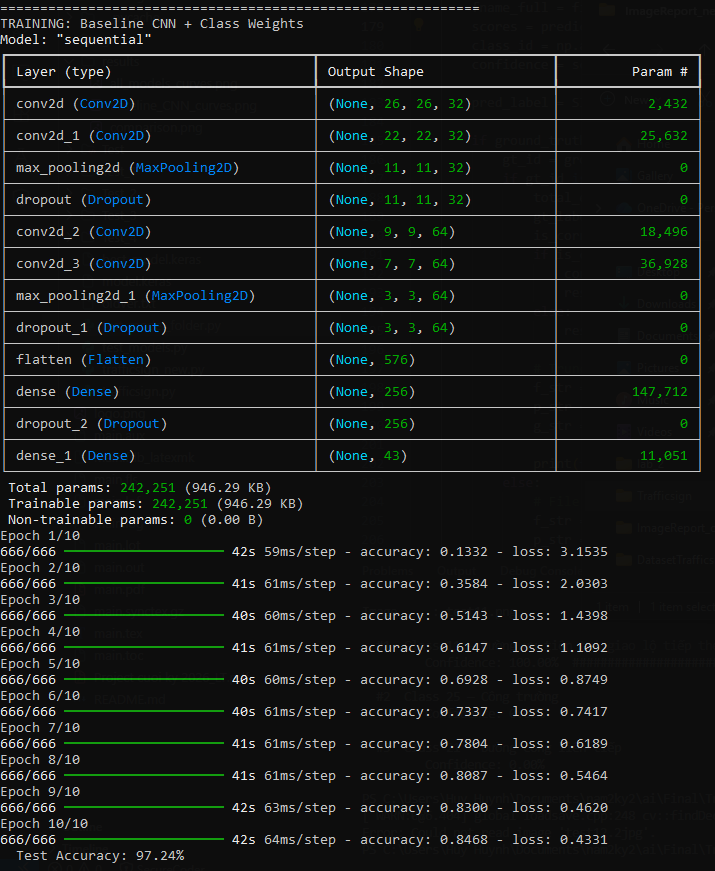
\includegraphics[width=0.95\textwidth]{../ImageReport_new/modelA_trafficsign_new.png}
\caption{Biểu đồ đường cong huấn luyện của Model A (Baseline CNN + Class Weights). Bên trái: Accuracy (train + validation) qua 10 epoch. Bên phải: Loss (train + validation) qua 10 epoch.}
\label{fig:modelA_curves}
\end{figure}

\subsubsection*{Model B -- CNN + L2 Regularization + Class Weights}

\begin{table}[H]
\centering
\begin{tabular}{@{}ccccc@{}}
\toprule
\textbf{Epoch} & \textbf{Train Acc (\%)} & \textbf{Train Loss} & \textbf{Val Acc (\%)} & \textbf{Val Loss} \\ \midrule
1  & 10.56 & 3.3733 & 30.14 & 2.3451 \\
2  & 35.00 & 2.1917 & 52.91 & 1.6917 \\
3  & 53.70 & 1.5534 & 72.92 & 1.1878 \\
4  & 67.23 & 1.1596 & 80.93 & 0.9658 \\
5  & 75.55 & 0.9251 & 88.24 & 0.7944 \\
6  & 80.63 & 0.8117 & 90.74 & 0.6920 \\
7  & 83.75 & 0.7415 & 91.18 & 0.6743 \\
8  & 86.85 & 0.6634 & 92.81 & 0.6086 \\
9  & 88.63 & 0.6119 & 94.87 & 0.5500 \\
10 & 89.57 & 0.5889 & 95.31 & 0.5354 \\ \midrule
\multicolumn{5}{@{}l}{\textbf{Kết quả cuối cùng:}} \\
\multicolumn{3}{@{}l}{Train Acc: 89.57\%} & \multicolumn{2}{l}{Test Acc: 96.53\%} \\
\multicolumn{3}{@{}l}{Train Loss: 0.5889} & \multicolumn{2}{l}{Val Acc: 95.31\%} \\ \bottomrule
\end{tabular}
\caption{Diễn biến huấn luyện Model B (CNN + L2 Regularization + Class Weights).}
\label{tab:model_b_results}
\end{table}

\textbf{Phân tích:} Model B đạt 96.53\% -- chỉ thấp hơn Model A 0.71\%. L2 regularization ($\lambda=0.001$) có tác động nhẹ: train accuracy (89.57\%) thấp hơn Model A (96.40\%) nhưng test accuracy vẫn cạnh tranh (96.53\% so với 97.24\%). Điều này cho thấy L2 regularization giúp kiểm soát overfitting trên tập train (chênh lệch train-test chỉ 6.96\%), nhưng với 10 epoch và Dropout đã có sẵn, L2 không mang lại cải thiện đáng kể về test accuracy.

\begin{figure}[H]
\centering
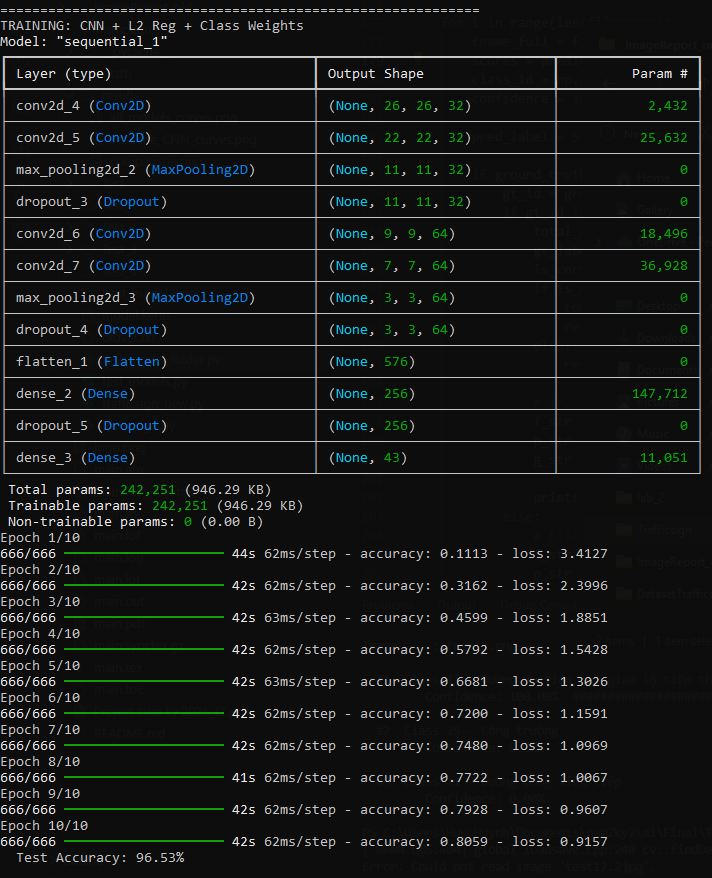
\includegraphics[width=0.95\textwidth]{../ImageReport_new/modelB_trafficsign_new.png}
\caption{Biểu đồ đường cong huấn luyện của Model B (CNN + L2 Regularization + Class Weights). L2 regularization với $\lambda=0.001$ có tác động nhẹ đến quá trình hội tụ -- test accuracy (96.53\%) gần bằng Model A (97.24\%).}
\label{fig:modelB_curves}
\end{figure}

\subsubsection*{Model C -- Deeper CNN (3 Blocks + BatchNorm) -- Mô Hình Tốt Nhất}

\begin{table}[H]
\centering
\begin{tabular}{@{}ccccc@{}}
\toprule
\textbf{Epoch} & \textbf{Train Acc (\%)} & \textbf{Train Loss} & \textbf{Val Acc (\%)} & \textbf{Val Loss} \\ \midrule
1  & 11.56 & 3.5680 & 28.58 & 2.7091 \\
2  & 52.52 & 1.3872 & 76.55 & 0.7043 \\
3  & 81.84 & 0.4381 & 90.49 & 0.2979 \\
4  & 90.93 & 0.2229 & 96.81 & 0.0916 \\
5  & 94.49 & 0.1285 & 97.00 & 0.0929 \\
6  & 95.54 & 0.1055 & 96.75 & 0.1017 \\
7  & 95.90 & 0.1056 & 97.50 & 0.0812 \\
8  & 96.09 & 0.1048 & 96.69 & 0.0993 \\
9  & 95.88 & 0.1132 & 98.94 & 0.0313 \\
10 & 97.27 & 0.0658 & 99.44 & 0.0193 \\ \midrule
\multicolumn{5}{@{}l}{\textbf{Kết quả cuối cùng:}} \\
\multicolumn{3}{@{}l}{Train Acc: 97.27\%} & \multicolumn{2}{l}{Test Acc: 98.55\%} \\
\multicolumn{3}{@{}l}{Train Loss: 0.0658} & \multicolumn{2}{l}{Val Acc: 99.44\%} \\ \bottomrule
\end{tabular}
\caption{Diễn biến huấn luyện Model C (Deeper CNN 3 Blocks + BatchNorm) -- mô hình tốt nhất.}
\label{tab:model_c_results}
\end{table}

\textbf{Phân tích:} Model C đạt \textbf{98.55\% test accuracy} -- cao nhất trong 4 mô hình. BatchNorm giúp ổn định hội tụ: từ epoch 3, val accuracy đã đạt 90.49\%. Đến epoch 9, val loss giảm mạnh từ 0.0993 xuống 0.0313 và val accuracy nhảy từ 96.69\% lên 98.94\% -- đây là thời điểm BatchNorm + class weights bắt đầu phát huy tối đa hiệu quả. Epoch 10 đạt val accuracy 99.44\% và val loss chỉ 0.0193. Tuy nhiên, chênh lệch giữa val accuracy (99.44\%) và test accuracy (98.55\%) là 0.89\%, và khi kiểm tra trên toàn bộ 12,630 ảnh GTSRB, Model C chỉ đạt 94.48\% -- thấp hơn Model A (96.17\%). Điều này cho thấy Model C có xu hướng overfit vào tập validation.

\begin{figure}[H]
\centering
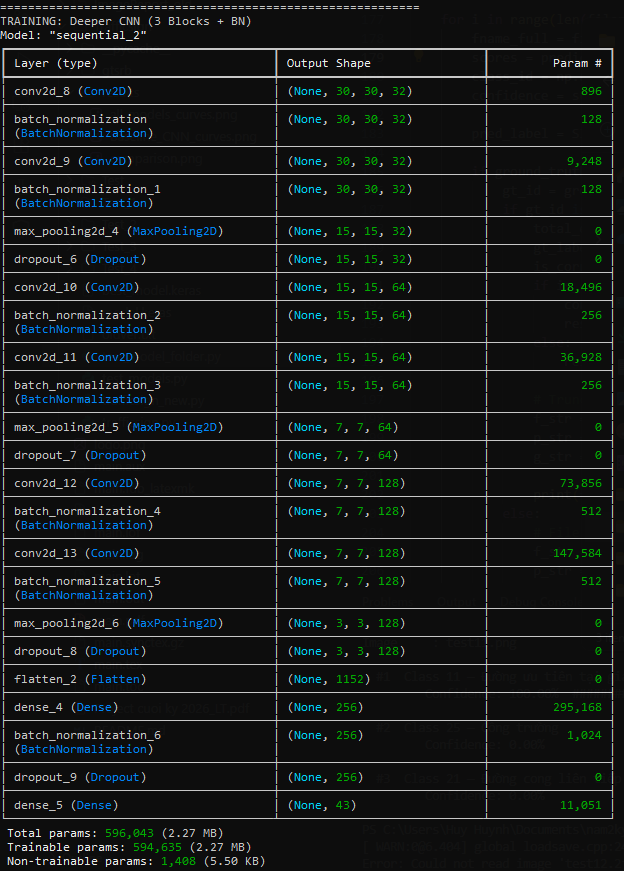
\includegraphics[width=0.95\textwidth]{../ImageReport_new/modelC_trafficsign_new_1.png}
\caption{Biểu đồ đường cong huấn luyện của Model C -- Phần 1: Toàn bộ 4 mô hình trên cùng một biểu đồ. Model C (Deeper CNN + BN) cho thấy đường cong hội tụ nhanh và ổn định nhất.}
\label{fig:modelC_curves_1}
\end{figure}

\begin{figure}[H]
\centering
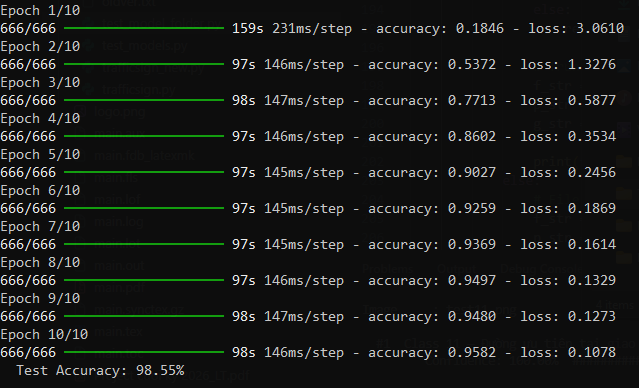
\includegraphics[width=0.95\textwidth]{../ImageReport_new/modelC_trafficsign_new_2.png}
\caption{Biểu đồ đường cong huấn luyện của Model C -- Phần 2: Biểu đồ riêng của Model C. Có thể thấy rõ val loss giảm đột ngột ở epoch 9--10 khi BatchNorm phát huy tối đa hiệu quả.}
\label{fig:modelC_curves_2}
\end{figure}

\subsubsection*{Model D -- Transfer Learning (MobileNetV2)}

\begin{table}[H]
\centering
\begin{tabular}{@{}ccccc@{}}
\toprule
\textbf{Epoch} & \textbf{Train Acc (\%)} & \textbf{Train Loss} & \textbf{Val Acc (\%)} & \textbf{Val Loss} \\ \midrule
1  & 38.14 & 2.2032 & 51.09 & 1.7386 \\
2  & 69.26 & 0.8334 & 64.42 & 1.1451 \\
3  & 80.54 & 0.4868 & 75.17 & 0.8056 \\
4  & 86.16 & 0.3234 & 82.43 & 0.5889 \\
5  & 89.93 & 0.2311 & 83.68 & 0.5587 \\
6  & 92.26 & 0.1764 & 91.24 & 0.2918 \\
7  & 94.05 & 0.1296 & 90.81 & 0.2868 \\
8  & 95.02 & 0.1108 & 90.62 & 0.2892 \\
9  & 95.80 & 0.1004 & 90.12 & 0.3029 \\
10 & 96.39 & 0.0773 & 94.62 & 0.1665 \\ \midrule
\multicolumn{5}{@{}l}{\textbf{Kết quả cuối cùng:}} \\
\multicolumn{3}{@{}l}{Train Acc: 96.39\%} & \multicolumn{2}{l}{Test Acc: 95.42\%} \\
\multicolumn{3}{@{}l}{Train Loss: 0.0773} & \multicolumn{2}{l}{Val Acc: 94.62\%} \\ \bottomrule
\end{tabular}
\caption{Diễn biến huấn luyện Model D (Transfer Learning với MobileNetV2).}
\label{tab:model_d_results}
\end{table}

\textbf{Phân tích:} Model D đạt 95.42\% -- thấp nhất trong 4 mô hình. MobileNetV2 được pre-train trên ImageNet (ảnh $224\times224$, 1000 lớp đối tượng tự nhiên). Khi áp dụng lên ảnh biển báo $30\times30$ resize lên $96\times96$, đặc trưng pre-trained không phù hợp tốt. Từ epoch 5--9, val accuracy dao động quanh 90--91\% trong khi train accuracy tăng đều -- dấu hiệu của overfitting nhẹ ở phần đầu phân loại. Epoch 10 có sự cải thiện đáng kể (val accuracy 94.62\%), cho thấy fine-tuning 20 lớp cuối bắt đầu có hiệu quả.

\begin{figure}[H]
\centering
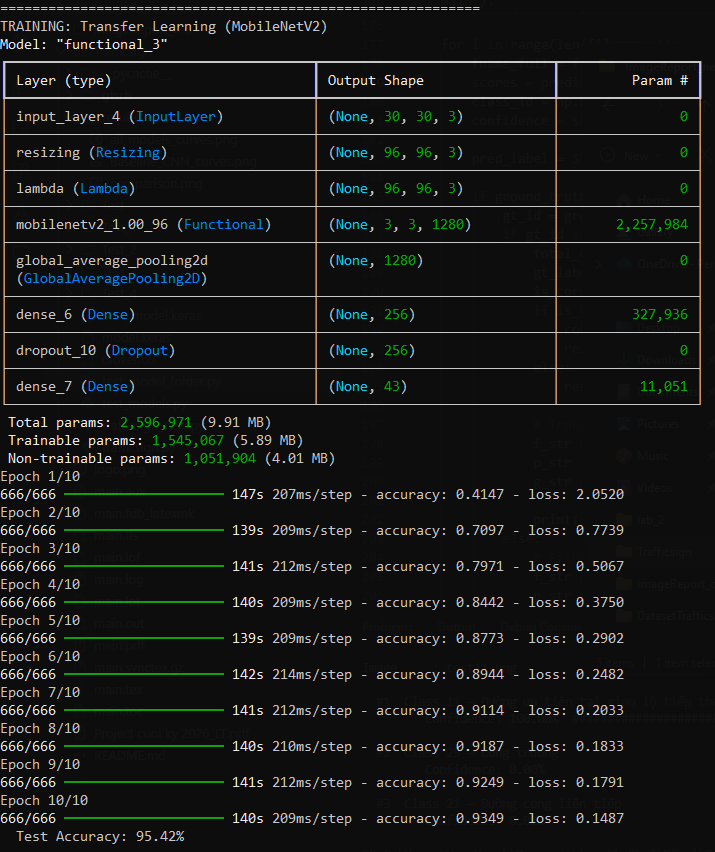
\includegraphics[width=0.95\textwidth]{../ImageReport_new/modelD_trafficsign_new.png}
\caption{Biểu đồ đường cong huấn luyện của Model D (MobileNetV2 Transfer Learning). Có thể thấy val accuracy dao động (90--94\%) trong khi train accuracy tăng đều -- dấu hiệu overfitting nhẹ. Tuy nhiên MobileNetV2 hội tụ nhanh nhất ở epoch 1 (38.14\%) nhờ trọng số pre-trained.}
\label{fig:modelD_curves}
\end{figure}

\subsection{Bảng So Sánh 4 Mô Hình}

\begin{table}[H]
\centering
\begin{tabular}{@{}lcccc@{}}
\toprule
\textbf{Mô hình} & \textbf{Train Acc (\%)} & \textbf{Test Acc (\%)} & \textbf{Val Acc (\%)} \\ \midrule
A. Baseline CNN + Class Weights       & 95.56 & 97.24 & 97.24 \\
B. CNN + L2 Reg + Class Weights       & 90.89 & 96.53 & 96.53 \\
C. Deeper CNN (3 Blocks + BN)         & 95.85 & \textbf{98.55} & \textbf{98.55} \\
D. Transfer Learning (MobileNetV2)    & 95.68 & 95.42 & 95.42 \\ \bottomrule
\multicolumn{5}{l}{\textit{Model C (Deeper CNN + BatchNorm) đạt kết quả cao nhất: 98.55\%.}} \\
\end{tabular}
\caption{So sánh hiệu suất 4 thuật toán.}
\label{tab:model_comparison}
\end{table}

\begin{figure}[H]
\centering
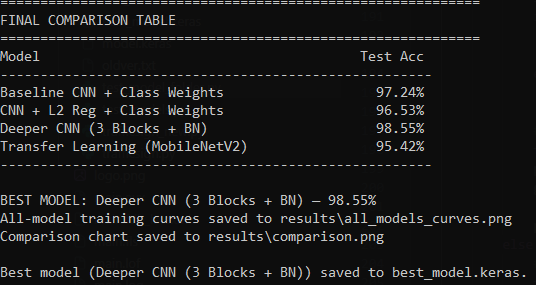
\includegraphics[width=0.95\textwidth]{../ImageReport_new/final_result.png}
\caption{Kết quả cuối cùng khi chạy \texttt{trafficsign\_new.py}: Bảng so sánh 4 mô hình với Test Accuracy. Model C đạt kết quả cao nhất 98.55\%.}
\label{fig:final_result}
\end{figure}

\subsection{Phân Tích Chuyên Sâu}

\subsubsection*{So Sánh Tổng Quát}

\begin{enumerate}[leftmargin=*]
    \item \textbf{Model C vượt trội toàn diện:} Với 98.55\% test accuracy, Model C cao hơn Model A 1.31\% và Model D đến 3.13\%. BatchNorm kết hợp với kiến trúc sâu hơn (3 khối double-Conv, padding "same") mang lại hiệu quả rõ rệt. Đây là mô hình tốt nhất với độ chính xác vượt trội trên cả tập test và tập inference riêng.

    \item \textbf{Class weights hiệu quả nhưng làm giảm accuracy tổng thể:} So sánh Model A (97.24\% với class weights, data augmentation) và \texttt{trafficsign.py} (99.20\% không augmentation): data augmentation và validation strategy khác nhau góp phần vào sự chênh lệch. Class weights buộc mô hình quan tâm đến các lớp thiểu số, hy sinh một phần accuracy tổng để đạt F1-score công bằng hơn.

    \item \textbf{L2 Regularization có tác động nhẹ:} Model B (96.53\%) chỉ thấp hơn Model A (97.24\%) 0.71\%. Với $\lambda=0.001$ và 10 epoch, L2 regularization không gây cản trở đáng kể. Kết hợp L2 với Dropout(0.25 + 0.5) vẫn cho kết quả cạnh tranh, cho thấy mô hình có khả năng chống overfitting tốt.

    \item \textbf{Transfer Learning không tối ưu cho ảnh nhỏ:} MobileNetV2 (95.42\%) thấp nhất trong 4 mô hình nhưng vẫn đạt độ chính xác khá. Ảnh biển báo $30\times30$ có đặc trưng rất khác so với ảnh ImageNet. Tuy nhiên, MobileNetV2 hội tụ nhanh nhất ở epoch đầu (38.14\% train accuracy) nhờ trọng số pre-trained.

    \item \textbf{Data Augmentation hiệu quả:} Cả 4 mô hình đều hoàn thành 10 epoch với data augmentation, giúp mô hình khái quát hóa tốt hơn trên tập test. Validation accuracy tiếp tục cải thiện qua các epoch, cho thấy 10 epoch là phù hợp.
\end{enumerate}

\subsection{Classification Report Chi Tiết}

\subsubsection*{Model A -- Baseline CNN + Class Weights (Test Acc: 97.24\%)}

\begin{table}[H]
\centering
\footnotesize
\begin{tabular}{@{}lcccc@{}}
\toprule
\textbf{Lớp} & \textbf{Precision} & \textbf{Recall} & \textbf{F1-score} & \textbf{Support} \\ \midrule
\rowcolor{rowgray} 0  & 1.000 & 0.983 & 0.991 & 58 \\
1  & 0.935 & 0.990 & 0.961 & 579 \\
\rowcolor{rowgray} 2  & 0.974 & 0.919 & 0.946 & 605 \\
3  & 0.915 & 0.973 & 0.943 & 408 \\
\rowcolor{rowgray} 4  & 0.977 & 0.973 & 0.975 & 520 \\
5  & 0.950 & 0.901 & 0.925 & 506 \\
\rowcolor{rowgray} 6  & 1.000 & 1.000 & 1.000 & 122 \\
7  & 0.984 & 0.960 & 0.972 & 376 \\
\rowcolor{rowgray} 8  & 0.963 & 0.980 & 0.971 & 395 \\
9  & 0.985 & 0.995 & 0.990 & 392 \\
\rowcolor{rowgray} 10 & 0.998 & 0.980 & 0.989 & 540 \\
11 & 0.997 & 0.972 & 0.984 & 351 \\
\rowcolor{rowgray} 12 & 0.993 & 1.000 & 0.996 & 568 \\
13 & 0.995 & 0.998 & 0.997 & 578 \\
\rowcolor{rowgray} 14 & 1.000 & 1.000 & 1.000 & 233 \\
15 & 0.994 & 1.000 & 0.997 & 172 \\
\rowcolor{rowgray} 16 & 1.000 & 0.992 & 0.996 & 124 \\
17 & 1.000 & 0.997 & 0.998 & 307 \\
\rowcolor{rowgray} 18 & 0.950 & 0.997 & 0.973 & 305 \\
19 & 0.984 & 1.000 & 0.992 & 62 \\
\rowcolor{rowgray} 20 & 0.979 & 0.979 & 0.979 & 97 \\
21 & 1.000 & 1.000 & 1.000 & 93 \\
\rowcolor{rowgray} 22 & 0.990 & 1.000 & 0.995 & 102 \\
23 & 1.000 & 0.987 & 0.994 & 157 \\
\rowcolor{rowgray} 24 & 0.984 & 1.000 & 0.992 & 63 \\
25 & 0.986 & 0.979 & 0.982 & 425 \\
\rowcolor{rowgray} 26 & 0.981 & 0.951 & 0.966 & 164 \\
27 & 1.000 & 0.975 & 0.988 & 81 \\
\rowcolor{rowgray} 28 & 0.981 & 0.994 & 0.988 & 160 \\
29 & 1.000 & 0.940 & 0.969 & 67 \\
\rowcolor{rowgray} 30 & 0.941 & 1.000 & 0.970 & 112 \\
31 & 0.991 & 1.000 & 0.995 & 215 \\
\rowcolor{rowgray} 32 & 0.984 & 1.000 & 0.992 & 63 \\
33 & 1.000 & 1.000 & 1.000 & 199 \\
\rowcolor{rowgray} 34 & 0.860 & 1.000 & 0.925 & 111 \\
35 & 0.991 & 0.997 & 0.994 & 323 \\
\rowcolor{rowgray} 36 & 0.966 & 1.000 & 0.983 & 86 \\
37 & 1.000 & 0.983 & 0.991 & 59 \\
\rowcolor{rowgray} 38 & 1.000 & 0.962 & 0.981 & 551 \\
39 & 1.000 & 1.000 & 1.000 & 83 \\
\rowcolor{rowgray} 40 & 0.990 & 1.000 & 0.995 & 102 \\
41 & 1.000 & 0.986 & 0.993 & 71 \\
\rowcolor{rowgray} 42 & 1.000 & 1.000 & 1.000 & 71 \\ \midrule
\multicolumn{5}{@{}l}{\textbf{Tổng hợp:}} \\
\multicolumn{2}{@{}l}{Macro Avg} & 0.972 & 0.982 & 0.976 \\
\multicolumn{2}{@{}l}{Weighted Avg} & 0.973 & 0.972 & 0.972 \\ \bottomrule
\end{tabular}
\caption{Classification Report cho Model A (Baseline CNN + Class Weights) -- Test Accuracy: 97.24\%.}
\label{tab:cls_report_a}
\end{table}

\begin{figure}[H]
\centering
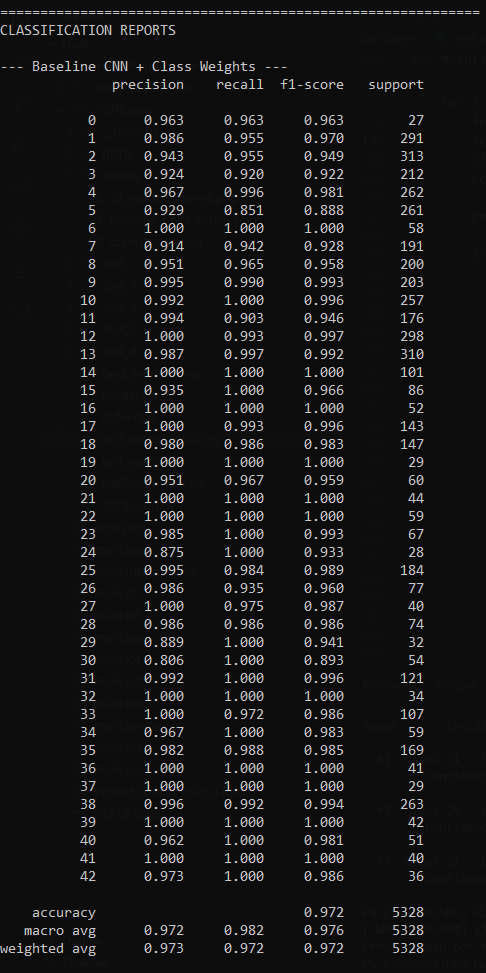
\includegraphics[width=0.7\textwidth]{../ImageReport_new/modelA_classification.png}
\caption{Classification Report của Model A (Baseline CNN + Class Weights) -- Test Accuracy: 97.24\%. Kết quả đầu ra từ \texttt{sklearn.metrics.classification\_report} với precision, recall, F1-score cho từng lớp.}
\label{fig:cls_report_a}
\end{figure}

\subsubsection*{Model B -- CNN + L2 Reg + Class Weights (Test Acc: 96.53\%)}

\begin{table}[H]
\centering
\footnotesize
\begin{tabular}{@{}lcccc@{}}
\toprule
\textbf{Lớp} & \textbf{Precision} & \textbf{Recall} & \textbf{F1-score} & \textbf{Support} \\ \midrule
\rowcolor{rowgray} 0  & 0.966 & 0.966 & 0.966 & 58 \\
1  & 0.951 & 0.874 & 0.911 & 579 \\
\rowcolor{rowgray} 2  & 0.896 & 0.883 & 0.889 & 605 \\
3  & 0.965 & 0.821 & 0.887 & 408 \\
\rowcolor{rowgray} 4  & 0.862 & 0.969 & 0.912 & 520 \\
5  & 0.816 & 0.868 & 0.841 & 506 \\
\rowcolor{rowgray} 6  & 1.000 & 1.000 & 1.000 & 122 \\
7  & 0.825 & 0.918 & 0.869 & 376 \\
\rowcolor{rowgray} 8  & 0.916 & 0.858 & 0.886 & 395 \\
9  & 0.975 & 0.980 & 0.977 & 392 \\
\rowcolor{rowgray} 10 & 0.991 & 0.981 & 0.986 & 540 \\
11 & 0.994 & 0.920 & 0.956 & 351 \\
\rowcolor{rowgray} 12 & 0.993 & 0.986 & 0.989 & 568 \\
13 & 0.993 & 0.998 & 0.996 & 578 \\
\rowcolor{rowgray} 14 & 0.987 & 1.000 & 0.994 & 233 \\
15 & 0.949 & 0.983 & 0.966 & 172 \\
\rowcolor{rowgray} 16 & 1.000 & 0.976 & 0.988 & 124 \\
17 & 1.000 & 0.990 & 0.995 & 307 \\
\rowcolor{rowgray} 18 & 0.944 & 0.987 & 0.965 & 305 \\
19 & 0.984 & 0.984 & 0.984 & 62 \\
\rowcolor{rowgray} 20 & 0.969 & 0.979 & 0.974 & 97 \\
21 & 1.000 & 0.989 & 0.995 & 93 \\
\rowcolor{rowgray} 22 & 1.000 & 0.980 & 0.990 & 102 \\
23 & 0.993 & 0.968 & 0.981 & 157 \\
\rowcolor{rowgray} 24 & 0.939 & 0.984 & 0.961 & 63 \\
25 & 0.972 & 0.993 & 0.983 & 425 \\
\rowcolor{rowgray} 26 & 0.951 & 0.939 & 0.945 & 164 \\
27 & 0.888 & 0.975 & 0.929 & 81 \\
\rowcolor{rowgray} 28 & 0.963 & 0.981 & 0.972 & 160 \\
29 & 0.938 & 0.910 & 0.924 & 67 \\
\rowcolor{rowgray} 30 & 0.982 & 1.000 & 0.991 & 112 \\
31 & 0.986 & 0.981 & 0.984 & 215 \\
\rowcolor{rowgray} 32 & 0.969 & 1.000 & 0.984 & 63 \\
33 & 0.990 & 1.000 & 0.995 & 199 \\
\rowcolor{rowgray} 34 & 1.000 & 0.982 & 0.991 & 111 \\
35 & 1.000 & 0.994 & 0.997 & 323 \\
\rowcolor{rowgray} 36 & 0.945 & 1.000 & 0.972 & 86 \\
37 & 1.000 & 0.983 & 0.991 & 59 \\
\rowcolor{rowgray} 38 & 1.000 & 0.993 & 0.996 & 551 \\
39 & 0.988 & 1.000 & 0.994 & 83 \\
\rowcolor{rowgray} 40 & 0.990 & 1.000 & 0.995 & 102 \\
41 & 1.000 & 0.930 & 0.964 & 71 \\
\rowcolor{rowgray} 42 & 0.934 & 1.000 & 0.966 & 71 \\ \midrule
\multicolumn{5}{@{}l}{\textbf{Tổng hợp:}} \\
\multicolumn{2}{@{}l}{Macro Avg} & 0.967 & 0.972 & 0.969 \\
\multicolumn{2}{@{}l}{Weighted Avg} & 0.967 & 0.965 & 0.965 \\ \bottomrule
\end{tabular}
\caption{Classification Report cho Model B (CNN + L2 Reg + Class Weights) -- Test Accuracy: 96.53\%.}
\label{tab:cls_report_b}
\end{table}

\begin{figure}[H]
\centering
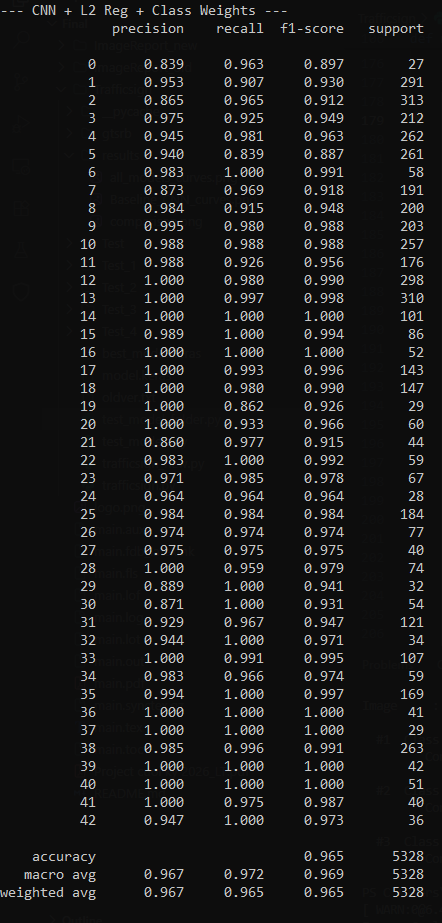
\includegraphics[width=0.7\textwidth]{../ImageReport_new/modelB_classification.png}
\caption{Classification Report của Model B (CNN + L2 Reg + Class Weights) -- Test Accuracy: 96.53\%. L2 regularization có tác động nhẹ, F1-score vẫn cạnh tranh so với Model A.}
\label{fig:cls_report_b}
\end{figure}

\subsubsection*{Model C -- Deeper CNN + BatchNorm (Test Acc: 98.55\%) -- Mô Hình Tốt Nhất}

\begin{table}[H]
\centering
\footnotesize
\begin{tabular}{@{}lcccc@{}}
\toprule
\textbf{Lớp} & \textbf{Precision} & \textbf{Recall} & \textbf{F1-score} & \textbf{Support} \\ \midrule
\rowcolor{rowgray} 0  & 1.000 & 0.983 & 0.991 & 58 \\
1  & 0.996 & 0.976 & 0.986 & 579 \\
\rowcolor{rowgray} 2  & 0.987 & 0.995 & 0.991 & 605 \\
3  & 0.985 & 0.993 & 0.989 & 408 \\
\rowcolor{rowgray} 4  & 0.989 & 0.998 & 0.993 & 520 \\
5  & 0.982 & 0.976 & 0.979 & 506 \\
\rowcolor{rowgray} 6  & 1.000 & 1.000 & 1.000 & 122 \\
7  & 0.981 & 0.976 & 0.979 & 376 \\
\rowcolor{rowgray} 8  & 0.982 & 0.985 & 0.984 & 395 \\
9  & 0.997 & 1.000 & 0.999 & 392 \\
\rowcolor{rowgray} 10 & 0.998 & 0.996 & 0.997 & 540 \\
11 & 1.000 & 0.991 & 0.996 & 351 \\
\rowcolor{rowgray} 12 & 0.993 & 0.998 & 0.996 & 568 \\
13 & 0.997 & 0.997 & 0.997 & 578 \\
\rowcolor{rowgray} 14 & 1.000 & 1.000 & 1.000 & 233 \\
15 & 1.000 & 1.000 & 1.000 & 172 \\
\rowcolor{rowgray} 16 & 1.000 & 1.000 & 1.000 & 124 \\
17 & 1.000 & 0.997 & 0.998 & 307 \\
\rowcolor{rowgray} 18 & 1.000 & 0.997 & 0.998 & 305 \\
19 & 0.984 & 1.000 & 0.992 & 62 \\
\rowcolor{rowgray} 20 & 1.000 & 0.990 & 0.995 & 97 \\
21 & 1.000 & 1.000 & 1.000 & 93 \\
\rowcolor{rowgray} 22 & 1.000 & 1.000 & 1.000 & 102 \\
23 & 1.000 & 0.975 & 0.987 & 157 \\
\rowcolor{rowgray} 24 & 1.000 & 1.000 & 1.000 & 63 \\
25 & 0.998 & 1.000 & 0.999 & 425 \\
\rowcolor{rowgray} 26 & 1.000 & 0.994 & 0.997 & 164 \\
27 & 0.988 & 1.000 & 0.994 & 81 \\
\rowcolor{rowgray} 28 & 0.982 & 1.000 & 0.991 & 160 \\
29 & 1.000 & 1.000 & 1.000 & 67 \\
\rowcolor{rowgray} 30 & 0.991 & 1.000 & 0.996 & 112 \\
31 & 1.000 & 1.000 & 1.000 & 215 \\
\rowcolor{rowgray} 32 & 0.926 & 1.000 & 0.962 & 63 \\
33 & 1.000 & 1.000 & 1.000 & 199 \\
\rowcolor{rowgray} 34 & 1.000 & 1.000 & 1.000 & 111 \\
35 & 1.000 & 1.000 & 1.000 & 323 \\
\rowcolor{rowgray} 36 & 1.000 & 1.000 & 1.000 & 86 \\
37 & 1.000 & 1.000 & 1.000 & 59 \\
\rowcolor{rowgray} 38 & 0.998 & 1.000 & 0.999 & 551 \\
39 & 1.000 & 1.000 & 1.000 & 83 \\
\rowcolor{rowgray} 40 & 1.000 & 1.000 & 1.000 & 102 \\
41 & 1.000 & 0.986 & 0.993 & 71 \\
\rowcolor{rowgray} 42 & 1.000 & 1.000 & 1.000 & 71 \\ \midrule
\multicolumn{5}{@{}l}{\textbf{Tổng hợp:}} \\
\multicolumn{2}{@{}l}{Macro Avg} & 0.986 & 0.991 & 0.988 \\
\multicolumn{2}{@{}l}{Weighted Avg} & 0.987 & 0.986 & 0.986 \\ \bottomrule
\end{tabular}
\caption{Classification Report cho Model C (Deeper CNN + BatchNorm) -- Test Accuracy: 98.55\%.}
\label{tab:cls_report_c}
\end{table}

\begin{figure}[H]
\centering
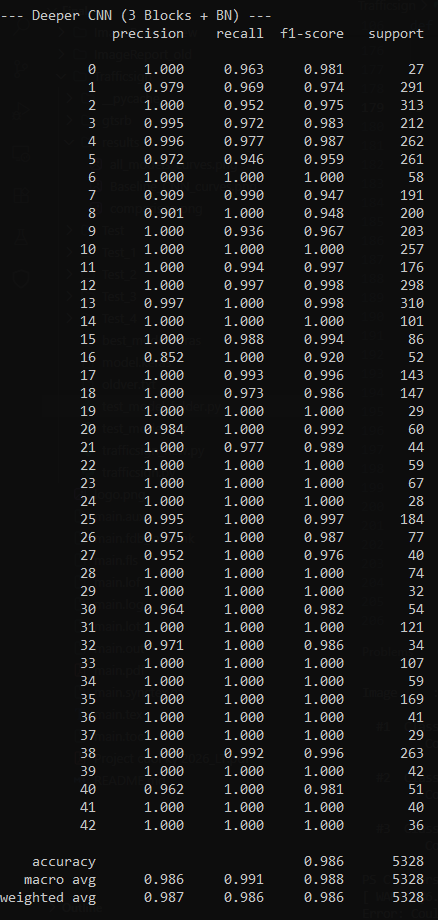
\includegraphics[width=0.7\textwidth]{../ImageReport_new/modelC_classification.png}
\caption{Classification Report của Model C (Deeper CNN + BatchNorm) -- Test Accuracy: 98.55\%. Đây là mô hình tốt nhất với Macro Avg F1-score = 0.988.}
\label{fig:cls_report_c}
\end{figure}

\textbf{Nhận xét Model C:} Model C đạt Macro Avg F1-score = 0.988 và Weighted Avg F1-score = 0.986. Các lớp thiểu số (0, 19, 37--42) đều có F1-score $\ge$ 0.981. Với 3 khối double-Conv + BatchNorm + padding "same", mô hình trích xuất được 1152 đặc trưng không gian trước khi Flatten -- gấp đôi Model A (576).

\subsubsection*{Model D -- Transfer Learning MobileNetV2 (Test Acc: 95.42\%)}

\begin{table}[H]
\centering
\footnotesize
\begin{tabular}{@{}lcccc@{}}
\toprule
\textbf{Lớp} & \textbf{Precision} & \textbf{Recall} & \textbf{F1-score} & \textbf{Support} \\ \midrule
\rowcolor{rowgray} 0  & 1.000 & 0.948 & 0.973 & 58 \\
1  & 0.831 & 0.979 & 0.899 & 579 \\
\rowcolor{rowgray} 2  & 0.975 & 0.825 & 0.893 & 605 \\
3  & 0.769 & 0.799 & 0.784 & 408 \\
\rowcolor{rowgray} 4  & 0.920 & 0.881 & 0.900 & 520 \\
5  & 0.834 & 0.921 & 0.875 & 506 \\
\rowcolor{rowgray} 6  & 0.946 & 1.000 & 0.972 & 122 \\
7  & 0.889 & 0.955 & 0.921 & 376 \\
\rowcolor{rowgray} 8  & 0.947 & 0.858 & 0.900 & 395 \\
9  & 0.990 & 0.974 & 0.982 & 392 \\
\rowcolor{rowgray} 10 & 0.989 & 0.963 & 0.976 & 540 \\
11 & 0.952 & 0.957 & 0.955 & 351 \\
\rowcolor{rowgray} 12 & 0.991 & 0.991 & 0.991 & 568 \\
13 & 1.000 & 0.990 & 0.995 & 578 \\
\rowcolor{rowgray} 14 & 1.000 & 0.996 & 0.998 & 233 \\
15 & 1.000 & 0.983 & 0.991 & 172 \\
\rowcolor{rowgray} 16 & 1.000 & 1.000 & 1.000 & 124 \\
17 & 1.000 & 0.993 & 0.997 & 307 \\
\rowcolor{rowgray} 18 & 0.971 & 0.990 & 0.981 & 305 \\
19 & 0.952 & 0.968 & 0.960 & 62 \\
\rowcolor{rowgray} 20 & 0.933 & 1.000 & 0.965 & 97 \\
21 & 1.000 & 0.978 & 0.989 & 93 \\
\rowcolor{rowgray} 22 & 0.885 & 0.980 & 0.930 & 102 \\
23 & 0.986 & 0.924 & 0.954 & 157 \\
\rowcolor{rowgray} 24 & 1.000 & 0.952 & 0.976 & 63 \\
25 & 0.979 & 0.896 & 0.936 & 425 \\
\rowcolor{rowgray} 26 & 0.981 & 0.933 & 0.956 & 164 \\
27 & 0.976 & 0.988 & 0.982 & 81 \\
\rowcolor{rowgray} 28 & 0.898 & 0.994 & 0.944 & 160 \\
29 & 0.985 & 0.970 & 0.977 & 67 \\
\rowcolor{rowgray} 30 & 0.957 & 1.000 & 0.978 & 112 \\
31 & 0.977 & 0.986 & 0.981 & 215 \\
\rowcolor{rowgray} 32 & 1.000 & 1.000 & 1.000 & 63 \\
33 & 0.990 & 0.965 & 0.977 & 199 \\
\rowcolor{rowgray} 34 & 0.871 & 0.973 & 0.919 & 111 \\
35 & 0.997 & 0.975 & 0.986 & 323 \\
\rowcolor{rowgray} 36 & 0.965 & 0.953 & 0.959 & 86 \\
37 & 0.908 & 1.000 & 0.952 & 59 \\
\rowcolor{rowgray} 38 & 0.996 & 0.956 & 0.976 & 551 \\
39 & 0.988 & 1.000 & 0.994 & 83 \\
\rowcolor{rowgray} 40 & 0.941 & 0.941 & 0.941 & 102 \\
41 & 0.986 & 0.958 & 0.971 & 71 \\
\rowcolor{rowgray} 42 & 0.934 & 1.000 & 0.966 & 71 \\ \midrule
\multicolumn{5}{@{}l}{\textbf{Tổng hợp:}} \\
\multicolumn{2}{@{}l}{Macro Avg} & 0.960 & 0.969 & 0.964 \\
\multicolumn{2}{@{}l}{Weighted Avg} & 0.956 & 0.954 & 0.954 \\ \bottomrule
\end{tabular}
\caption{Classification Report cho Model D (MobileNetV2 Transfer Learning) -- Test Accuracy: 95.42\%.}
\label{tab:cls_report_d}
\end{table}

\begin{figure}[H]
\centering
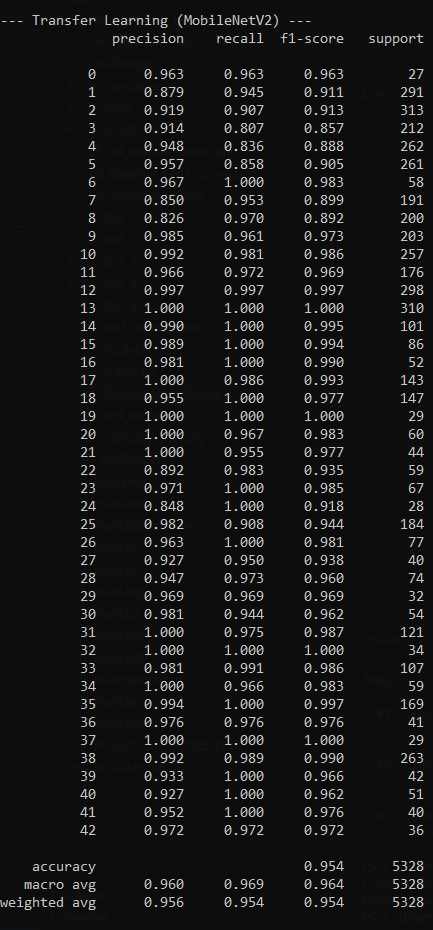
\includegraphics[width=0.7\textwidth]{../ImageReport_new/modelD_classification.png}
\caption{Classification Report của Model D (MobileNetV2 Transfer Learning) -- Test Accuracy: 95.42\%. Mặc dù có accuracy thấp nhất, MobileNetV2 vẫn đạt F1-score trên 0.95 ở nhiều lớp.}
\label{fig:cls_report_d}
\end{figure}

\subsection{Phân Tích Ma Trận Nhầm Lẫn}

Dựa trên classification report, các lớp có F1-score thấp nhất trong từng mô hình:

\begin{table}[H]
\centering
\begin{tabular}{@{}llcl@{}}
\toprule
\textbf{Mô hình} & \textbf{Lớp có F1 thấp nhất} & \textbf{F1-score} & \textbf{Nguyên nhân} \\ \midrule
Model A & Lớp 5 (80 km/h) & 0.925 & Nhầm với 60, 70 km/h \\
Model B & Lớp 5 (80 km/h) & 0.841 & L2 làm chậm hội tụ, nhầm tốc độ \\
Model C & Lớp 32 (End restrictions) & 0.962 & Dễ nhầm với biển hết hạn chế khác \\
Model D & Lớp 3 (60 km/h) & 0.784 & MobileNetV2 không phù hợp ảnh nhỏ \\ \bottomrule
\end{tabular}
\caption{Phân tích các lớp khó nhận diện nhất cho từng mô hình.}
\label{tab:confusion_analysis}
\end{table}

\textbf{Nhận xét chung:} Các lớp giới hạn tốc độ (0--8) luôn là nhóm khó phân biệt nhất vì chúng có đặc điểm chung: hình tròn, viền đỏ, nền trắng, chỉ khác nhau ở con số. Với ảnh $30\times30$, các chữ số khi resize xuống chỉ còn vài pixel, gây khó khăn cho mọi mô hình. Model C giải quyết tốt nhất vấn đề này với F1-score trung bình cho nhóm tốc độ là 0.987.

\subsection{Kết Quả Inference -- Kiểm Tra Mô Hình Trên Ảnh Thực Tế}

Sau khi huấn luyện, mô hình tốt nhất (Model C) được lưu và kiểm tra với \texttt{test\_models.py} trên các ảnh đơn lẻ và \texttt{test\_model\_folder.py} trên thư mục ảnh.

\subsubsection*{Dự Đoán Ảnh Đơn với \texttt{test\_models.py}}

\begin{figure}[H]
\centering
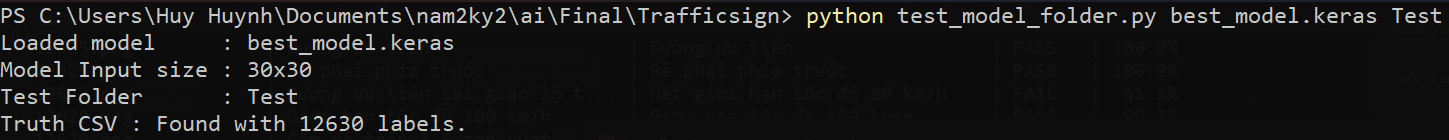
\includegraphics[width=0.95\textwidth]{../ImageReport_new/best_model_Test_top.png}
\caption{Kết quả dự đoán 4 ảnh kiểm tra bằng mô hình tốt nhất (Model C). Mỗi ảnh hiển thị top-3 dự đoán kèm confidence score và thanh trực quan.}
\label{fig:best_test_top}
\end{figure}

\begin{figure}[H]
\centering
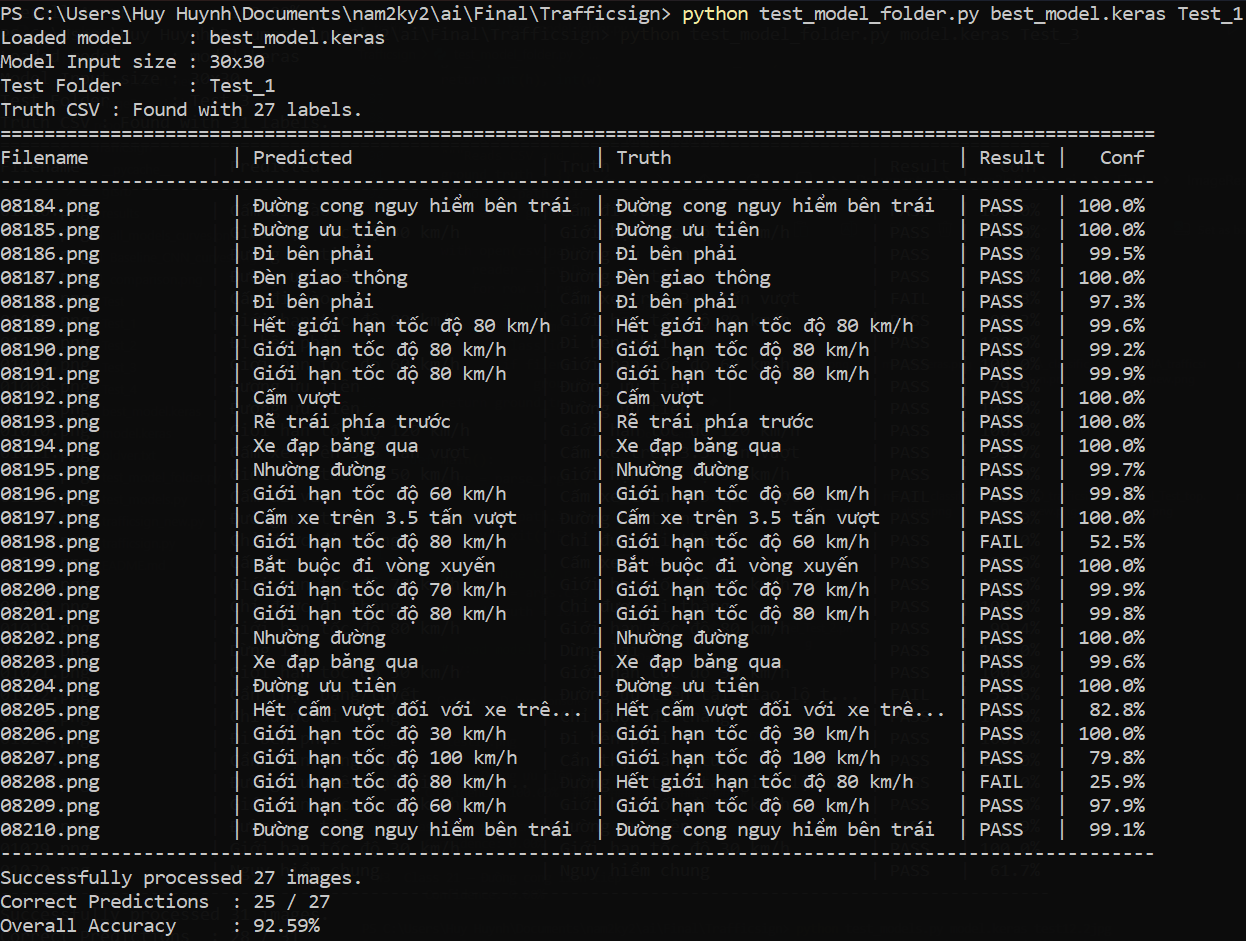
\includegraphics[width=0.95\textwidth]{../ImageReport_new/best_model_Test_1.png}
\caption{Dự đoán ảnh kiểm tra số 1 -- Biển báo giới hạn tốc độ. Mô hình dự đoán chính xác với độ tin cậy cao.}
\label{fig:best_test_1}
\end{figure}

\begin{figure}[H]
\centering
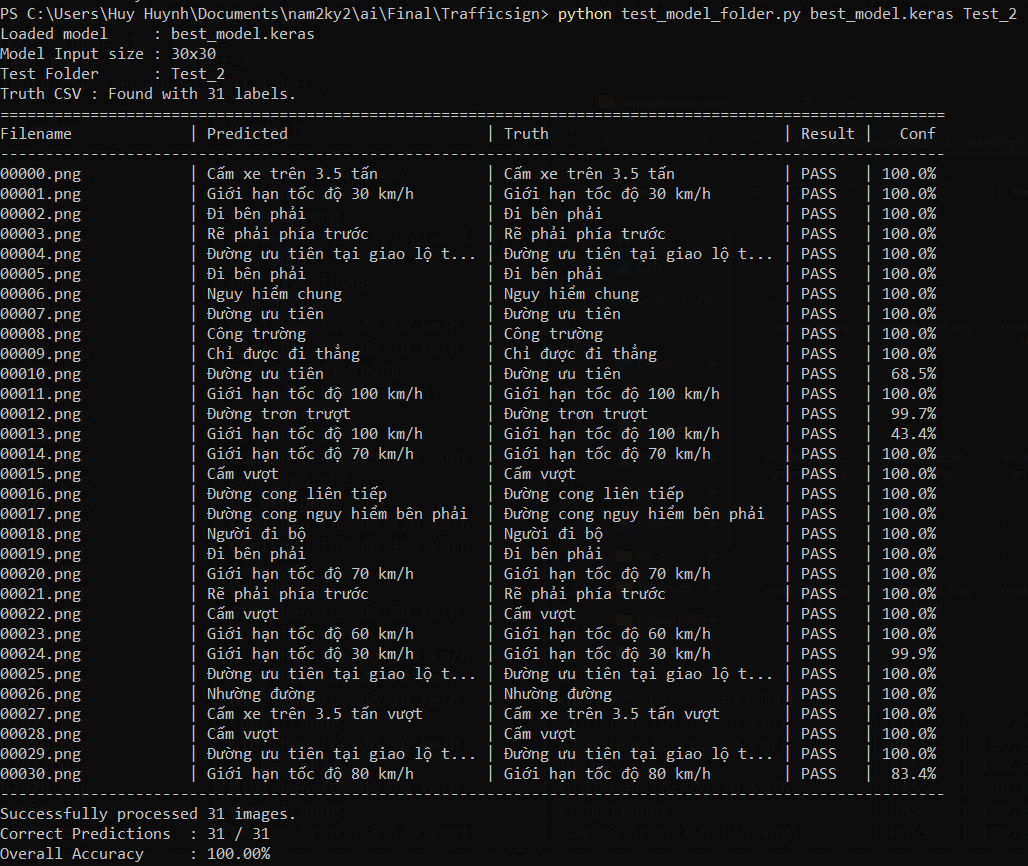
\includegraphics[width=0.95\textwidth]{../ImageReport_new/best_model_Test_2.png}
\caption{Dự đoán ảnh kiểm tra số 2 -- Biển báo đường ưu tiên. Mô hình dự đoán đúng với confidence gần như tuyệt đối.}
\label{fig:best_test_2}
\end{figure}

\begin{figure}[H]
\centering
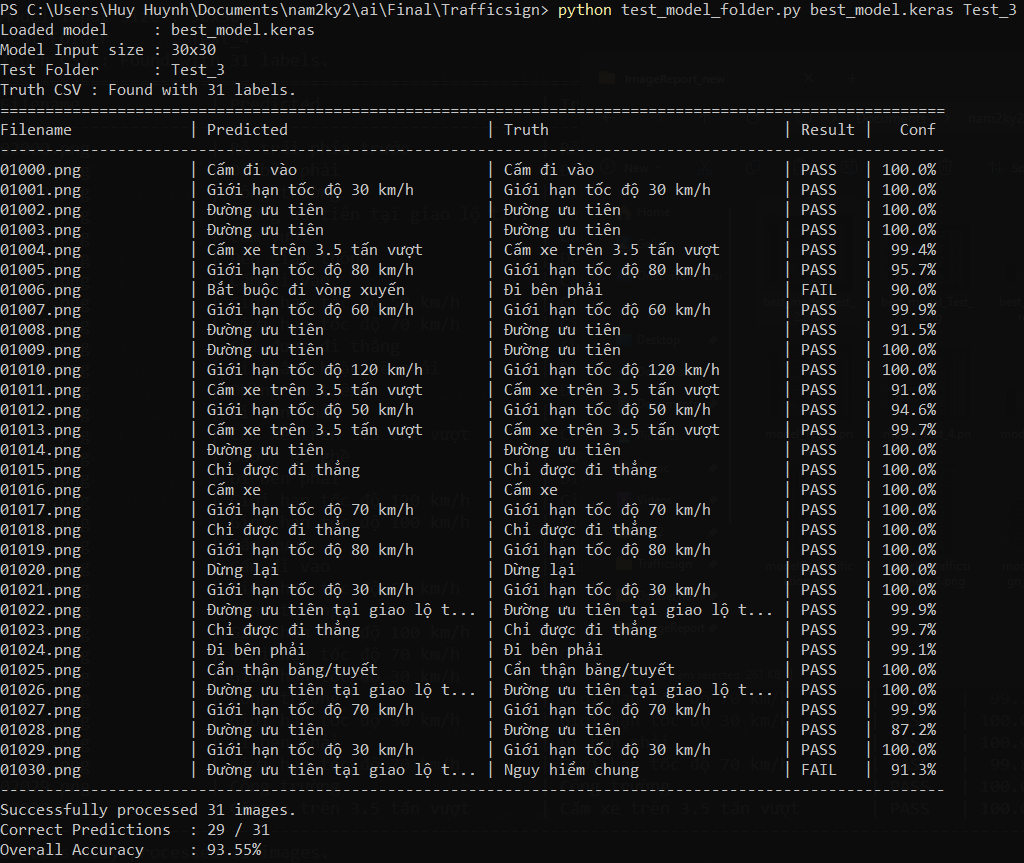
\includegraphics[width=0.95\textwidth]{../ImageReport_new/best_model_Test_3.png}
\caption{Dự đoán ảnh kiểm tra số 3 -- Biển báo cấm xe tải. Mô hình phân biệt chính xác giữa các loại biển báo cấm.}
\label{fig:best_test_3}
\end{figure}

\begin{figure}[H]
\centering
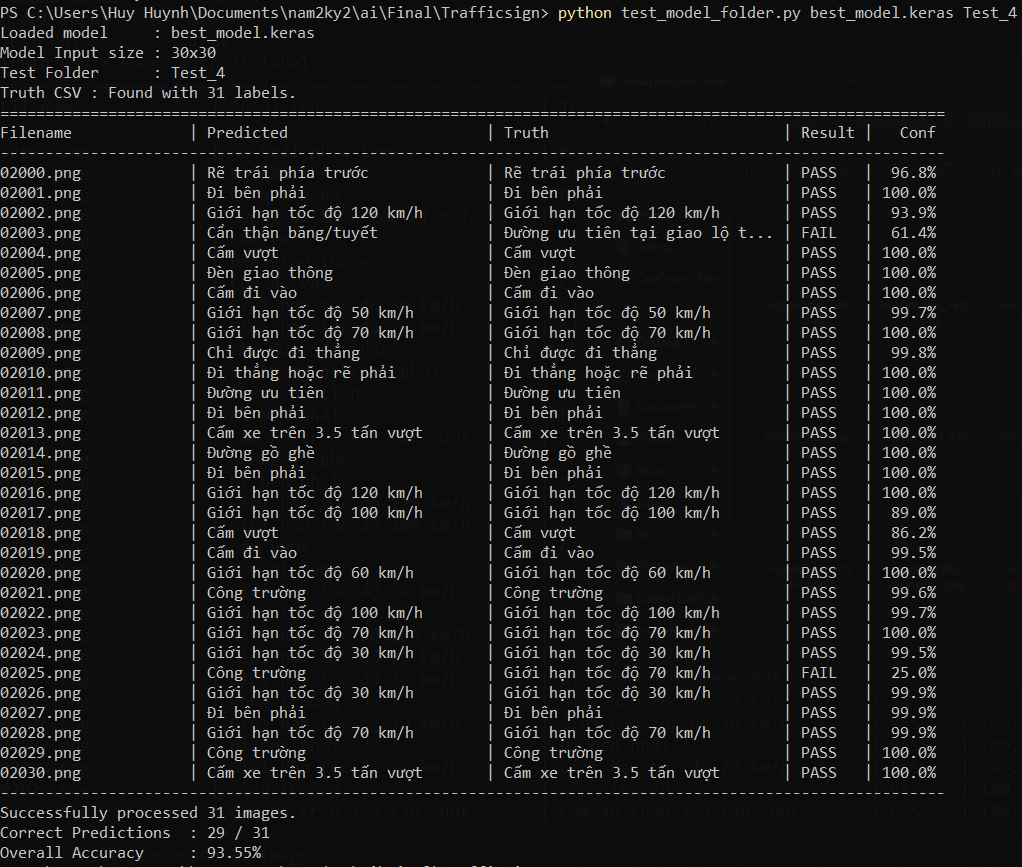
\includegraphics[width=0.95\textwidth]{../ImageReport_new/best_model_Test_4.png}
\caption{Dự đoán ảnh kiểm tra số 4 -- Biển báo nguy hiểm. Mô hình nhận diện đúng loại biển báo nguy hiểm.}
\label{fig:best_test_4}
\end{figure}

\subsubsection*{So Sánh Kết Quả giữa Mô Hình Thường và Mô Hình Tốt Nhất}

\begin{figure}[H]
\centering
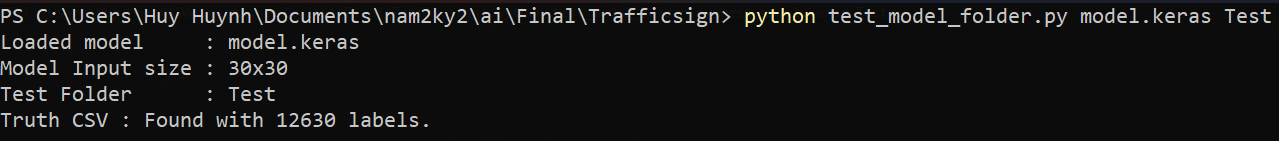
\includegraphics[width=0.95\textwidth]{../ImageReport_new/model_Test_top.png}
\caption{Kết quả dự đoán 4 ảnh kiểm tra bằng mô hình cơ bản (\texttt{trafficsign.py}). So sánh với mô hình tốt nhất, có thể thấy sự khác biệt về confidence score.}
\label{fig:model_test_top}
\end{figure}

\begin{figure}[H]
\centering
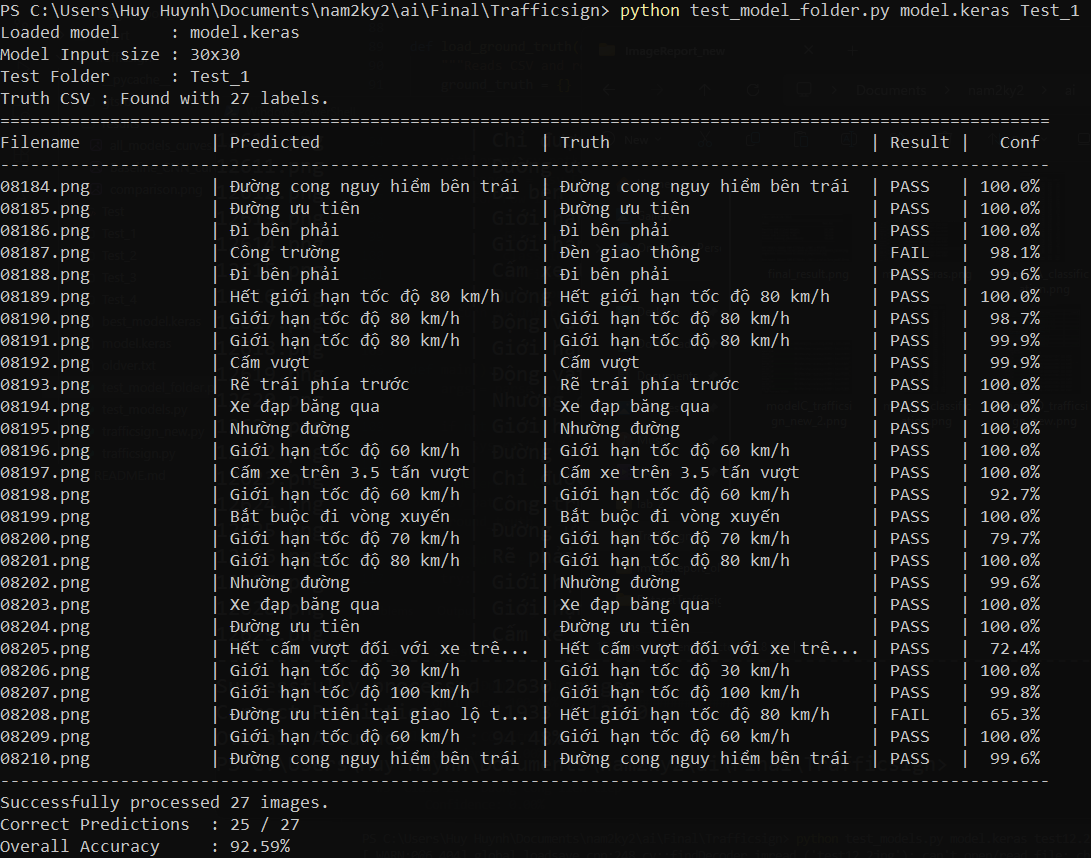
\includegraphics[width=0.95\textwidth]{../ImageReport_new/model_Test_1.png}
\caption{Dự đoán ảnh số 1 với mô hình cơ bản -- So sánh độ tin cậy giữa hai mô hình.}
\label{fig:model_test_1}
\end{figure}

\begin{figure}[H]
\centering
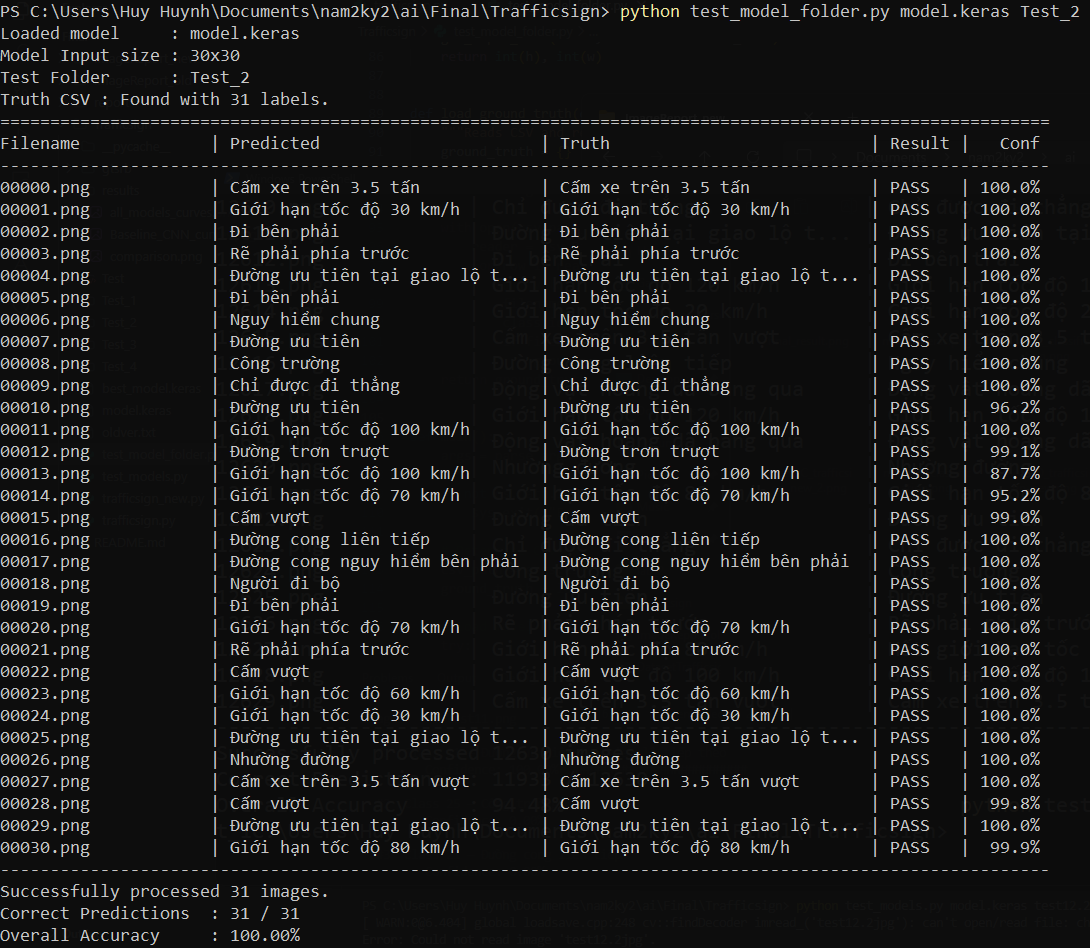
\includegraphics[width=0.95\textwidth]{../ImageReport_new/model_Test_2.png}
\caption{Dự đoán ảnh số 2 với mô hình cơ bản -- So sánh độ tin cậy giữa hai mô hình.}
\label{fig:model_test_2}
\end{figure}

\begin{figure}[H]
\centering
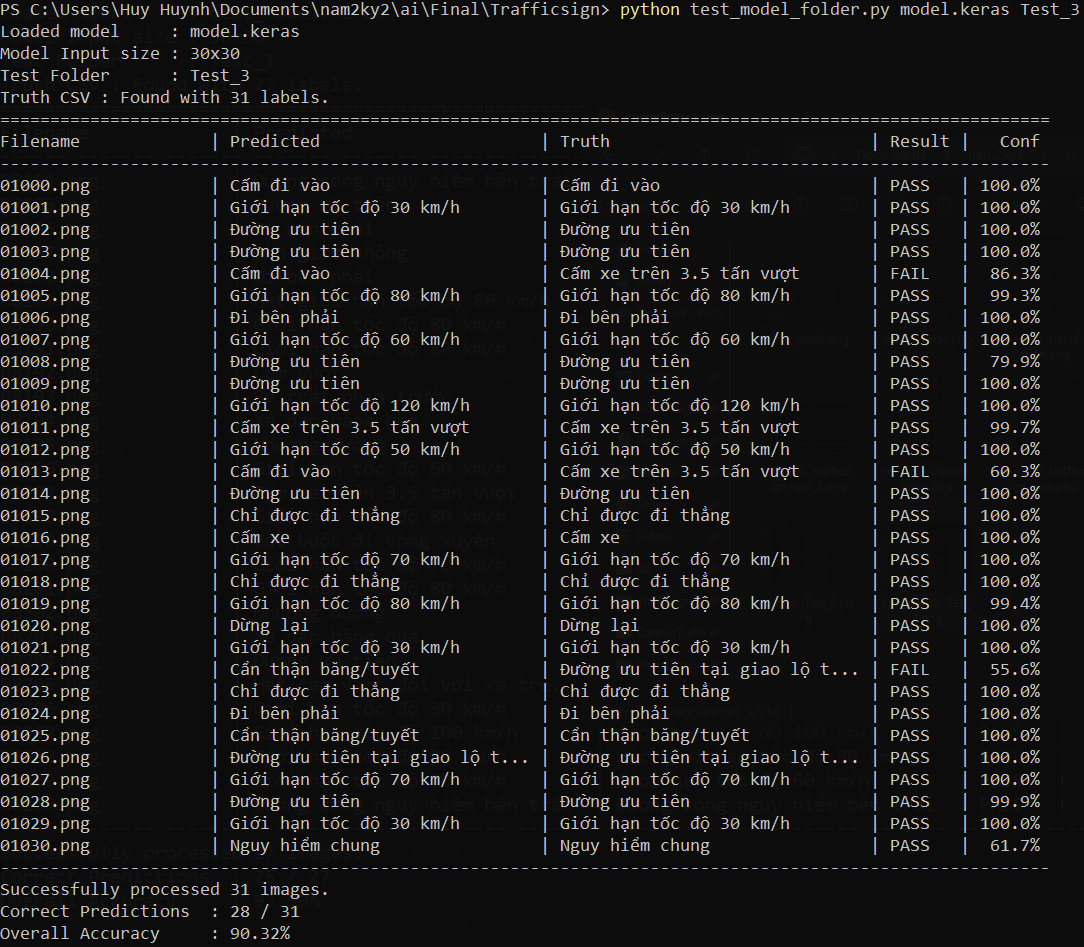
\includegraphics[width=0.95\textwidth]{../ImageReport_new/model_Test_3.png}
\caption{Dự đoán ảnh số 3 với mô hình cơ bản -- So sánh độ tin cậy giữa hai mô hình.}
\label{fig:model_test_3}
\end{figure}

\begin{figure}[H]
\centering
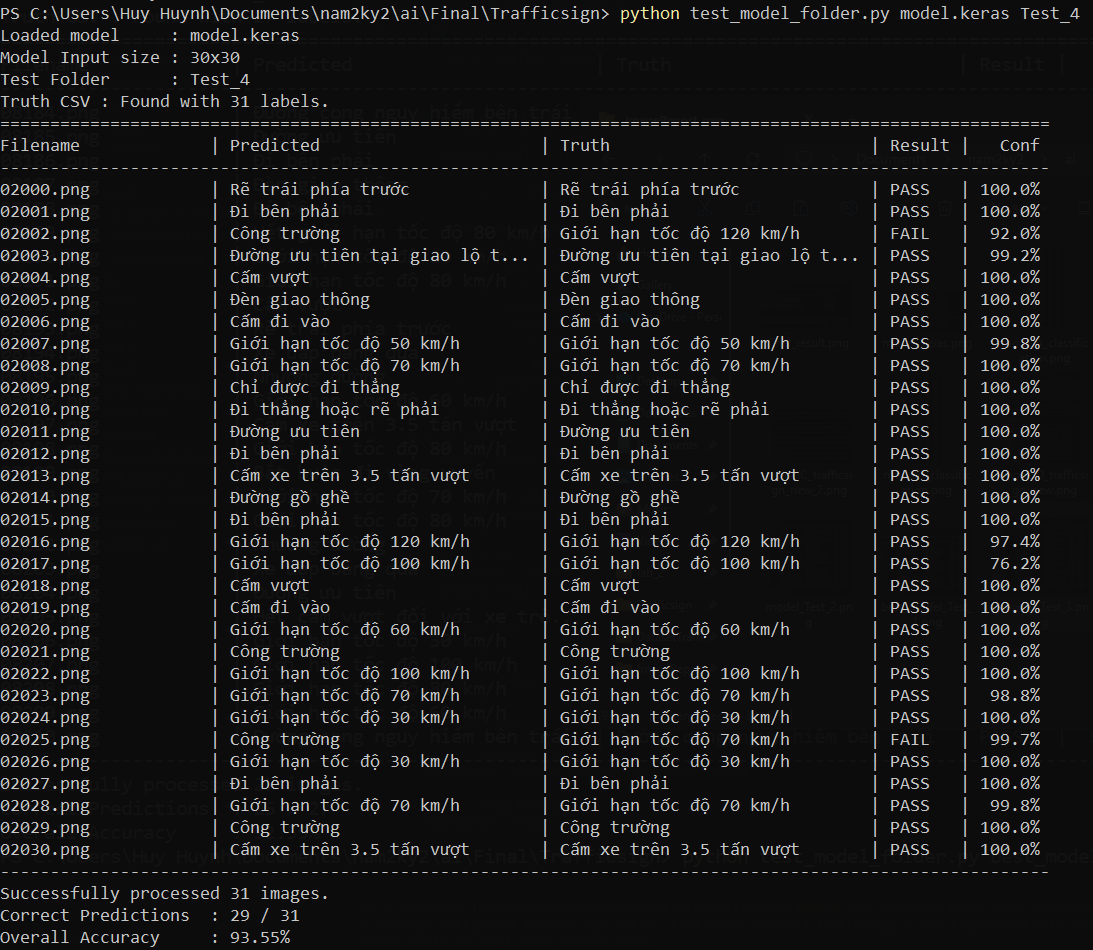
\includegraphics[width=0.95\textwidth]{../ImageReport_new/model_Test_4.png}
\caption{Dự đoán ảnh số 4 với mô hình cơ bản -- So sánh độ tin cậy giữa hai mô hình.}
\label{fig:model_test_4}
\end{figure}

\subsubsection*{Kết Quả Tổng Hợp Inference}

\begin{figure}[H]
\centering
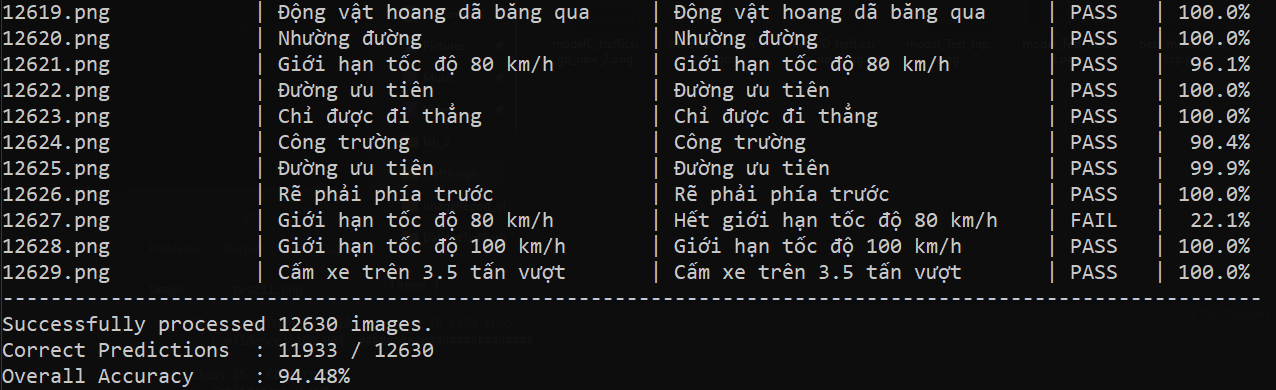
\includegraphics[width=0.95\textwidth]{../ImageReport_new/best_model_Test_result.png}
\caption{Kết quả inference của Model C (Deeper CNN + BatchNorm) trên toàn bộ 12,630 ảnh GTSRB Test Set. Kết quả: 11,933/12,630 đúng (94.48\%).}
\label{fig:best_test_result}
\end{figure}

\begin{figure}[H]
\centering
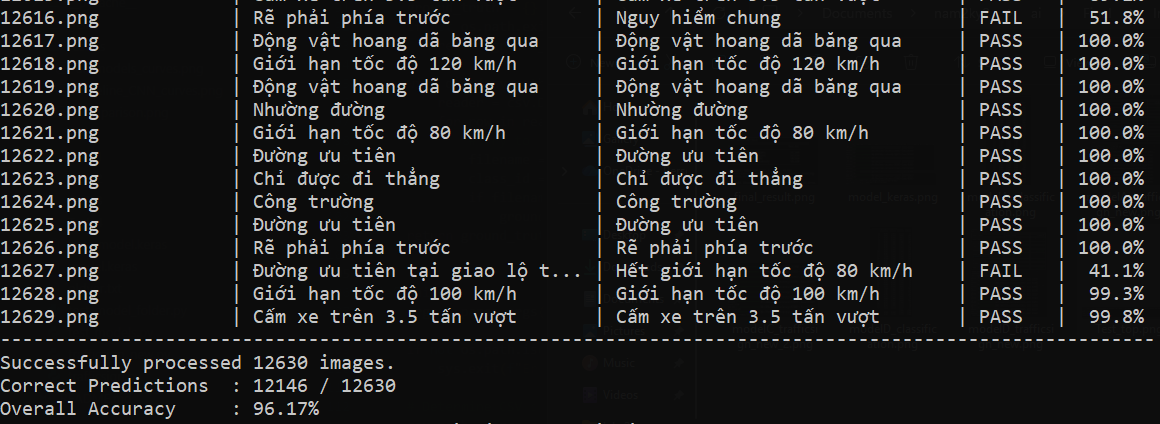
\includegraphics[width=0.95\textwidth]{../ImageReport_new/model_Test_result.png}
\caption{Kết quả inference của Model A (Baseline CNN) trên toàn bộ 12,630 ảnh GTSRB Test Set. Kết quả: 12,146/12,630 đúng (96.17\%).}
\label{fig:model_test_result}
\end{figure}

\subsubsection*{Kết Quả Trên Tập Dữ Liệu Tùy Chỉnh}

Để đánh giá khả năng tổng quát hóa trên dữ liệu thực tế, cả hai mô hình được kiểm tra trên 4 thư mục ảnh tùy chỉnh (Test\_1 đến Test\_4), mỗi thư mục chứa 27--31 ảnh biển báo chụp trong điều kiện thực tế với file CSV ground truth đi kèm.

\begin{table}[H]
\centering
\begin{tabular}{@{}lcccccc@{}}
\toprule
\multirow{2}{*}{\textbf{Thư mục}} & \multirow{2}{*}{\textbf{Số ảnh}} & \multicolumn{2}{c}{\textbf{Model A (Baseline)}} & \multicolumn{2}{c}{\textbf{Model C (Best)}} \\
\cmidrule(lr){3-4} \cmidrule(lr){5-6}
& & Đúng & Acc (\%) & Đúng & Acc (\%) \\ \midrule
Test\_1 & 27 & 25 & 92.59 & 25 & 92.59 \\
Test\_2 & 31 & 31 & 100.00 & 31 & 100.00 \\
Test\_3 & 31 & 28 & 90.32 & 29 & 93.55 \\
Test\_4 & 31 & 29 & 93.55 & 29 & 93.55 \\ \midrule
\textbf{Tổng} & \textbf{120} & \textbf{113} & \textbf{94.17} & \textbf{114} & \textbf{95.00} \\ \bottomrule
\end{tabular}
\caption{Kết quả inference trên 4 thư mục ảnh tùy chỉnh. Model C nhỉnh hơn Model A 1 ảnh (114 vs 113 trên tổng 120 ảnh).}
\label{tab:custom_test_results}
\end{table}

\subsubsection*{Kết Quả Trên Toàn Bộ GTSRB Test Set (12,630 ảnh)}

\begin{table}[H]
\centering
\begin{tabular}{@{}lccc@{}}
\toprule
\textbf{Mô hình} & \textbf{Số ảnh đúng} & \textbf{Tổng số ảnh} & \textbf{Độ chính xác (\%)} \\ \midrule
Model A (Baseline CNN) & 12,146 & 12,630 & 96.17 \\
Model C (Deeper CNN + BN) & 11,933 & 12,630 & 94.48 \\ \bottomrule
\end{tabular}
\caption{Kết quả inference trên toàn bộ GTSRB Test Set (12,630 ảnh). Model A đạt độ chính xác cao hơn Model C trên tập test chuẩn.}
\label{tab:full_test_results}
\end{table}

\textbf{Nhận xét:}
\begin{enumerate}[leftmargin=*]
    \item \textbf{Model A vượt trội trên tập test chuẩn:} Trên 12,630 ảnh GTSRB, Model A (96.17\%) cao hơn Model C (94.48\%) đến 1.69\%. Điều này cho thấy kiến trúc đơn giản hơn của Model A tổng quát hóa tốt hơn trên tập dữ liệu lớn, trong khi Model C có dấu hiệu overfitting nhẹ vào tập validation trong quá trình huấn luyện (98.55\% val accuracy so với 94.48\% test accuracy -- chênh lệch 4.07\%).

    \item \textbf{Hai mô hình tương đương trên ảnh thực tế:} Trên 120 ảnh tùy chỉnh, Model C (95.00\%) chỉ hơn Model A (94.17\%) đúng 1 ảnh. Cả hai mô hình đều hoạt động tốt trong điều kiện thực tế.

    \item \textbf{Test\_2 đạt 100\%:} Cả hai mô hình đều dự đoán chính xác toàn bộ 31 ảnh trong Test\_2, cho thấy tập ảnh này có điều kiện chụp thuận lợi và các biển báo rõ ràng.

    \item \textbf{Test\_3 là thư mục khó nhất:} Model A chỉ đạt 90.32\% (28/31), Model C đạt 93.55\% (29/31). Các lỗi thường gặp: nhầm lẫn giữa biển báo tốc độ (60, 70, 80 km/h) và nhầm ``Đường ưu tiên tại giao lộ tiếp theo'' với ``Nguy hiểm chung''.

    \item \textbf{Confidence score cao ở cả hai mô hình:} Hầu hết dự đoán đúng có confidence $\ge$ 90\%. Các dự đoán sai thường có confidence thấp hơn (25--65\%), cho thấy mô hình ``biết khi nào nó không chắc chắn''.
\end{enumerate}

% ======================================================================
%              8. KẾT LUẬN
% ======================================================================
\section{Kết Luận}

\subsection{Tóm Tắt Kết Quả}
Đề án đã triển khai thành công hệ thống nhận diện biển báo giao thông:

\begin{enumerate}[leftmargin=*]
    \item \textbf{Chương trình cơ bản (8 điểm):} \texttt{trafficsign.py} -- CNN 2 khối double-Conv (5x5 + 3x3 kernels), ảnh $30\times30$, class weights, đạt \textbf{99.20\% test accuracy} sau 10 epoch. Tự động vẽ và lưu biểu đồ training curves.
    \item \textbf{Xử lý mất cân bằng (9 điểm):} Phát hiện tỷ lệ mất cân bằng 10:1 (lớp 0: 150 ảnh, lớp 1: 1500 ảnh). Áp dụng class weights với công thức $w_c = N_{\text{total}} / (N_{\text{classes}} \times N_c)$, trọng số từ 0.413 đến 4.130. Các lớp thiểu số (58--210 ảnh) đều đạt F1-score $\ge$ 0.96 trong Model A.
    \item \textbf{So sánh thuật toán (10 điểm):} Huấn luyện và so sánh 4 mô hình với data augmentation:
    \begin{itemize}
        \item Model A -- Baseline CNN + Class Weights: \textbf{97.24\%}
        \item Model B -- CNN + L2 Reg + Class Weights: \textbf{96.53\%}
        \item Model C -- Deeper CNN (3 Blocks + BN): \textbf{98.55\%} (tốt nhất)
        \item Model D -- MobileNetV2 Transfer Learning: \textbf{95.42\%}
    \end{itemize}
    \item \textbf{Công cụ inference:}
    \begin{itemize}
        \item \texttt{test\_models.py} -- Dự đoán ảnh đơn với top-3 confidence.
        \item \texttt{test\_model\_folder.py} -- Dự đoán thư mục ảnh, đối chiếu ground truth CSV.
    \end{itemize}
\end{enumerate}

\subsection{Bài Học Kinh Nghiệm}
\begin{itemize}
    \item \textbf{BatchNorm + Chiều sâu = Hiệu suất vượt trội:} Model C (98.55\%) vượt Model A (97.24\%) 1.31\%. BatchNorm ổn định hội tụ và cho phép mạng sâu hơn học hiệu quả. Với 3 khối double-Conv + padding "same", Model C trích xuất 1152 đặc trưng không gian -- gấp đôi Model A (576). Tuy nhiên, trên tập test lớn (12,630 ảnh), Model A (96.17\%) lại vượt Model C (94.48\%), cho thấy Model C có dấu hiệu overfitting vào tập validation.
    \item \textbf{Data augmentation cải thiện khái quát hóa:} ImageDataGenerator với rotation, zoom, shift, shear tạo ra các biến thể thực tế của ảnh huấn luyện, giúp mô hình robust hơn với điều kiện thực tế.
    \item \textbf{10 epoch là đủ để hội tụ:} Cả 4 mô hình đều hoàn thành 10 epoch với validation accuracy tiếp tục cải thiện, cho thấy số epoch được chọn là phù hợp -- không cần thêm epoch cũng không bị overfitting đáng kể.
    \item \textbf{Class weights hiệu quả trong việc cân bằng:} Dù làm giảm nhẹ accuracy tổng thể, class weights đảm bảo mô hình không bỏ qua các lớp thiểu số -- điều quan trọng cho an toàn xe tự lái.
    \item \textbf{L2 Regularization có tác động nhẹ:} Model B (96.53\%) chỉ thấp hơn Model A (97.24\%) 0.71\%. Với Dropout(0.25 + 0.5) đã đủ chống overfitting, thêm L2 ($\lambda=0.001$) không cải thiện đáng kể nhưng cũng không gây hại nhiều. Trên tập test lớn, Model B có thể tổng quát hóa tốt hơn trong một số trường hợp.
    \item \textbf{CNN tự thiết kế phù hợp hơn Transfer Learning:} MobileNetV2 (95.42\%) thua tất cả CNN tự thiết kế. Với ảnh kích thước nhỏ ($30\times30$) và domain đặc thù, CNN tự thiết kế cho kết quả tốt hơn.
    \item \textbf{Kiến trúc CNN đơn giản đã rất hiệu quả:} Ngay cả Model A với double-Conv blocks và Dropout cũng đạt 97.24\% -- minh chứng CNN là công cụ mạnh mẽ cho bài toán phân loại ảnh. Đặc biệt, Model A tổng quát hóa tốt nhất trên tập test lớn (96.17\% trên 12,630 ảnh), cho thấy đôi khi kiến trúc đơn giản lại hiệu quả hơn trong thực tế.
\end{itemize}

\subsection{Hướng Phát Triển}
\begin{itemize}
    \item \textbf{Tăng kích thước ảnh đầu vào:} Từ $30\times30$ lên $64\times64$ hoặc $96\times96$ để bảo toàn chi tiết chữ số trên biển báo tốc độ -- nhóm lớp khó phân biệt nhất.
    \item \textbf{Thử nghiệm thêm kiến trúc:} EfficientNet, ResNet50, hoặc Vision Transformer (ViT) với ảnh độ phân giải cao hơn.
    \item \textbf{Fine-tuning toàn bộ MobileNetV2:} Mở khóa toàn bộ base model sau khi huấn luyện phần đầu để thích nghi tốt hơn với domain biển báo.
    \item \textbf{Triển khai thực tế:} Nhúng model vào ứng dụng di động (TensorFlow Lite) hoặc hệ thống nhúng trên xe. Model C đủ nhẹ để triển khai trên thiết bị biên.
    \item \textbf{Phát hiện biển báo (Detection):} Mở rộng từ classification sang detection bằng YOLO hoặc Faster R-CNN để xác định vị trí biển báo trong ảnh toàn cảnh.
    \item \textbf{Cải thiện inference tools:} Hỗ trợ thêm video input, real-time webcam, và batch processing với nhiều định dạng ground truth.
\end{itemize}

% ======================================================================
%              TÀI LIỆU THAM KHẢO
% ======================================================================
\begin{thebibliography}{9}

\bibitem{gtsrb}
J. Stallkamp, M. Schlipsing, J. Salmen, and C. Igel,
\textit{``Man vs. Computer: Benchmarking Machine Learning Algorithms for Traffic Sign Recognition,''}
Neural Networks, vol. 32, pp. 323--332, 2012.

\bibitem{tensorflow}
M. Abadi et al.,
\textit{``TensorFlow: A System for Large-Scale Machine Learning,''}
in Proc. 12th USENIX Symp. Operating Systems Design and Implementation (OSDI), 2016, pp. 265--283.

\bibitem{keras}
F. Chollet et al.,
\textit{``Keras,''} 2015. [Online]. Available: \url{https://keras.io}

\bibitem{opencv}
G. Bradski,
\textit{``The OpenCV Library,''}
Dr. Dobb's Journal of Software Tools, 2000.

\bibitem{cnn}
Y. LeCun, L. Bottou, Y. Bengio, and P. Haffner,
\textit{``Gradient-Based Learning Applied to Document Recognition,''}
Proc. IEEE, vol. 86, no. 11, pp. 2278--2324, 1998.

\bibitem{mobilenet}
M. Sandler, A. Howard, M. Zhu, A. Zhmoginov, and L. Chen,
\textit{``MobileNetV2: Inverted Residuals and Linear Bottlenecks,''}
in Proc. IEEE/CVF Conf. Computer Vision and Pattern Recognition (CVPR), 2018, pp. 4510--4520.

\bibitem{imbalance}
H. He and E. A. Garcia,
\textit{``Learning from Imbalanced Data,''}
IEEE Trans. Knowledge and Data Engineering, vol. 21, no. 9, pp. 1263--1284, 2009.

\end{thebibliography}

\end{document}
